\documentclass[11pt]{article}
\usepackage[margin=1in]{geometry}
\usepackage{array}
\usepackage{booktabs}
\usepackage{bm}
\usepackage{amsthm}
\usepackage{amsmath}
\usepackage{amstext}
\usepackage{amsfonts}
\usepackage{graphicx}
\usepackage{natbib}
\usepackage{lineno}
\usepackage{bbm}
\usepackage{xurl}
\usepackage{verbatim}
\usepackage{setspace}
\usepackage{breakurl}

\usepackage{hyperref}
\hypersetup{
  colorlinks=true,
  linkcolor=blue,
  citecolor=blue,
  urlcolor=blue}

\usepackage{verbatim}
%% R
\newcommand{\pkg}[1]{{\normalfont\fontseries{b}\selectfont #1}}
\let\proglang=\textsf
\let\code=\texttt

%% Cite options
\def\citeapos#1{\citeauthor{#1}'s (\citeyear{#1})}

%% Reduce Bibliography space
\usepackage{enumitem}
\bibpunct{(}{)}{;}{a}{,}{,}

\baselineskip = 7 mm
\parskip = 2.5 mm

\makeatletter
\renewcommand{\paragraph}{\@startsection{paragraph}{4}{0ex}%
   {-3.25ex plus -1ex minus -0.2ex}%
   {1.5ex plus 0.2ex}%
   {\normalfont\normalsize\bfseries}}
\makeatother

\begin{document}

\def\spacingset#1{\renewcommand{\baselinestretch}%
{#1}\small\normalsize} \spacingset{1.5}

\title{\bf Forecast combinations: \\Using multiple models to improve forecasts}

%\author{}
\maketitle

\bigskip
\begin{abstract}

\end{abstract}

\noindent%
{\it Keywords:}
\vfill

\bigskip

% \newpage
\spacingset{1.5}

\section{Introduction}
\label{sec:introduction}

Forecasting has risen to prominence as a tool that supports future-oriented decision making and strategic planning within the operational research community. Now rapid advances in computing motivate the explosive growth of methods for time series forecasting, including statistical and econometric models, machine learning algorithms, and even judgemental methods; see, e.g., \cite{De_Gooijer2006-eg} and \cite{Petropoulos2021-ft} for important and thorough reviews. Each of these methods has its own specialty and is developed with a separate assumption on the unknown data generation process (DGP) for the observed data. With such a diverse toolbox of forecasting methods, how can different aspects of the information be leveraged to achieve gains?

Combining forecasts derived from numerous forecasting methods is often considered as a successful alternative to identifying a single `best forecast'. Observed time series data are almost unlikely to be generated by a simple process specified with a functional form because of the possibility of time-varying trends, seasonality changes, structural breaks, etc. \citep{Clements1998-bu}. Thus, selecting a single `best model' for a given time series to approximate the unknown underlying DGP may be misleading and subject to three sources of uncertainty, namely data uncertainty, parameter uncertainty, and model uncertainty \citep{Petropoulos2018-fw,Kourentzes2019-na}. Such cases are common in forecasting applications and thus make forecast selection a challenging task in practice. Given these challenges, alternatively forecast combinations, which involve combining multiple forecasts to incorporate multiple drivers of the DGP and mitigate uncertainties regarding model form and parameter specification, are widely supported to avoid selecting a misspecified model; see, e.g., \cite{Kolassa2011-ai}, \cite{Chan2018-jl}, and \cite{Makridakis2020-hu} for theoretical investigation and empirical evidence in favour of forecast combination over selection.

Fifty years have passed since \citeapos{Bates1969-yj} seminal work on forecast combinations, also referred to as `ensembles', `aggregations', `model averages', etc. in different domains and applications. It is well established that forecast combinations are beneficial, offering substantially improved forecasts on average relative to constituent models; see \cite{Clemen1989-fb} and \cite{Timmermann2006-en} for exhaustive literature reviews. Further, a recent strand of the literature provides insights into the reasons for the success of forecast combinations and thus offers practical guidelines for their use \citep{Palm1992-im,De_Menezes2000-vd,Chan2018-jl,Atiya2020-ge,Lichtendahl2020-ut}. In light of the superiority, forecast combinations have made their appearance in a wide range of applications such as retail \citep{Ma2021-np}, energy \citep{Xie2016-fb}, economics \citep{Aastveit2018-lf}, and epidemiology \citep{Brooks2020-sg}. Among all forecasting papers published in the Web of Science, the proportion of papers that concern forecast combinations has revealed an overall upward trend over the past $50$ years, reaching $6.14\%$ in $2021$ as shown in Figure~\ref{fig:prop}. Thus, it is timely and necessary to review the extant literature on this topic. {\color{red} need to update}

\begin{figure}
  \centering 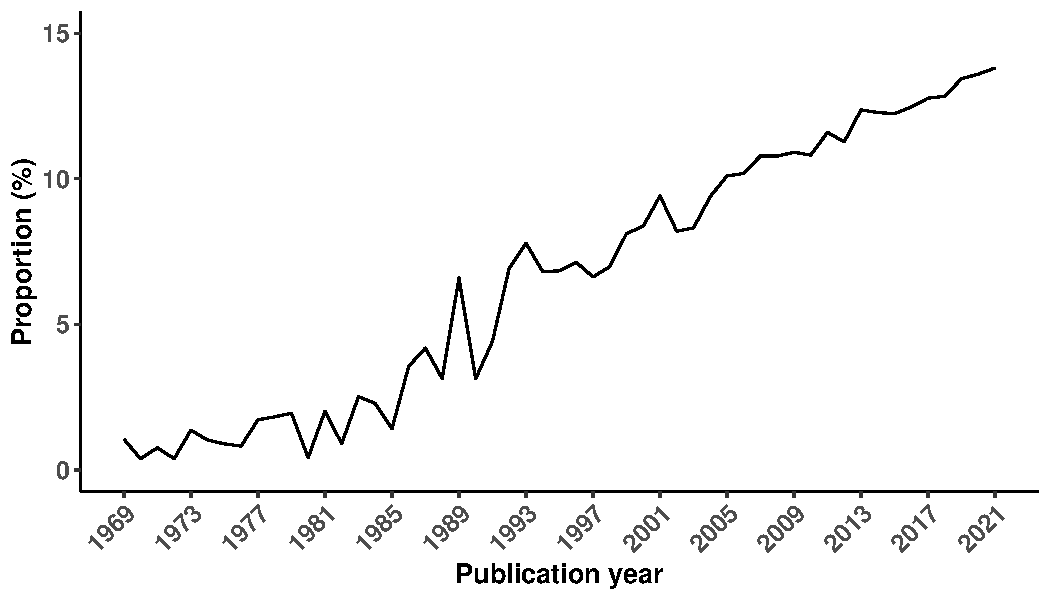
\includegraphics[width=0.85\textwidth]{prop}
  \caption{The proportion of papers that concern forecast combinations among all forecasting papers published in the Web of Science databases during the period $1972$-$2021$.}
  \label{fig:prop}
\end{figure}

The gains from forecast combinations highly rely on not only the quality of the individual forecasts to be combined but the estimation of the combination weights assigned to each forecast \citep{Timmermann2006-en,Cang2014-tp}. Numerous studies have devoted to discussing critical issues with respect to the constitution of the model pool, including but not limited to the accuracy, diversity, and robustness of individual models, and the selection of the optimal model subset \citep{Batchelor1995-ps,Mannes2014-dl,Thomson2019-al,Lichtendahl2020-ut,Kang2021-ol}. On the other hand, combination schemes vary across studies and evolve from simple combination methods that avoid weight estimation \citep[e.g.,][]{Clemen1986-pd,Palm1992-im,Genre2013-ut,Grushka-Cockayne2017-dj,Petropoulos2020-fp} to sophisticated methods that tailor weights for different individual models \citep[e.g.,][]{Bates1969-yj,Newbold1974-lp,Kolassa2011-ai,Li2020-od,Montero-Manso2020-tq,Kang2021-ol,Wang2021-un}. Accordingly, Forecast combinations can be linear or nonlinear, static or time-varying, series-specific or cross-learning, and ignore or cover the correlation among individual forecasts. Despite the diverse set of forecast combination schemes, forecasters still have little guidance on how to solve the `forecast combination puzzle' \citep{Stock2004-rq,Smith2009-wd,Claeskens2016-pv,Chan2018-jl}---simple averaging often dominates sophisticated weighting schemes that should theoretically be superior.

Initial work on forecast combinations focused on dealing with point forecasts since the seminal work of \cite{Bates1969-yj} \citep[see, for example,][]{Clemen1989-fb,Timmermann2006-en}. In recent years considerable attention has moved towards the use of probabilistic forecasts \citep[e.g.,][]{Hall2007-lh,Gneiting2013-hl,Kapetanios2015-bb,Martin2021-yi} as they enable the assessment of forecast uncertainties and provide decision makers with more insights to gain prominence in a variety of applications, ranging from macroeconomics to energy. When working with probabilistic forecasts, issues such as diversity among individual forecasts may be more complex and less understood than combining point forecasts \citep{Ranjan2010-jl} and additional issues such as calibration and sharpness need to be considered to help for an overall assessment and thus the selection of combination schemes \citep{Gneiting2007-fr}. Additionally, combining probabilistic forecasts elicited in different forms (i.e., probability forecasts and quantiles) will result in combined forecasts with completely different properties such as calibration, sharpness, and shape; see \cite{Lichtendahl2013-rt} for further analytical details.

The past five decades have seen growing interests in combining forecasts to achieve gains. This paper intends to present an up-to-date review of the literature on forecast combinations. The review will cover a wide variety of forecast combination methods for both point forecasts and probabilistic forecast, focusing on classifying them and highlighting how the various ideas have developed in parallel but are related. Comparisons between the reviewed combination methods in terms of advantages and disadvantages are also provided. Furthermore, some important issues concerning the competence of forecast combinations are also surveyed. Finally, we discuss current challenges and potential directions for future work.

We should clarify that we take the individual forecasts to be combined intrinsically as given and do not shed light on how the forecasts themselves are generated. Although the literature involves several other ways in which multiple forecasts or models get used for combinations, we only consider combinations of multiple forecasts directly derived from \textit{separate} and \textit{non-interfering} models for a given series. For example, we do not cover bootstrap aggregation (bagging), in which the remainder of a given series is bootstrapped to create multiple versions of the given series and multiple forecasts are produced thenceforth and aggregated to form the final forecast \citep[see, for example,][]{Bergmeir2016-ae,Petropoulos2018-fw}. The reviewed combination methods in this paper can then function as various tools to aggregate (combine) the produced multiple forecasts in this particular context. Moreover, the aim of the review is not to judge the superiority of any approaches, as different approaches should be tailored to specific forecasting problems, but rather to contribute a personal and historical overview of the main developments, even though there may be some important papers we have missed.

% Conclude with a brief paragraph that describes the organization of the rest of the paper.
The rest of this article is organized as follows:
% further identifies possible developments in the future.


%\section{Point forecasts}
%\label{sec:point_forecasts}

\section{Simple point forecast combinations}
\label{sec:simple_combinations}

Considerable literature has accumulated over the years regarding how individual forecasts are combined. A unanimous conclusion is that simple combination schemes are hard to beat \citep{Clemen1989-fb,Fischer1999-kz,Stock2004-rq,Lichtendahl2020-ut}. More specifically, simple combination rules which ignore past information regarding the precision of individual forecasts and correlations between forecast errors work reasonably well relative to more sophisticated combination schemes, as noted in \citeapos{Clemen1989-fb} survey. \cite{Lichtendahl2020-ut} attributed this phenomenon to a lower risk of simple combination methods resulting in bad forecasts than more sophisticated combination methods. \cite{Timmermann2006-en} concisely summarized the reasons for the success of simple combinations using the importance of parameter estimation error --- simple combination schemes did not require estimating parameters such as combination weights based on forecast errors, thus avoiding parameter estimation error that often existed in weighted combinations.

The vast majority of studies on combining multiple models have dealt with point forecasting, even though point forecasts generally provide insufficient information for decision making. The simple arithmetic average of forecasts based on equal weights stands out as the most popular and surprisingly robust combination rule \citep[see][]{Bunn1985-vo,Clemen1986-pd,Stock2003-sp,Genre2013-ut}. \cite{Makridakis1982-hb} reported the results of M-competition, a forecasting competition involving $1,001$ economic time series, and found that the simple average outperformed the individual techniques. \cite{Clemen1989-fb} provided an extensive bibliographical review of the early work on the combination of forecasts, and then addressed the issue that the arithmetic means often dominated more refined forecast combinations. \cite{Makridakis1983-hg} concluded empirically that a larger number of individual methods included in the simple average scheme would help improve the accuracy of combined forecasts and reduce the variability associated with the choice of methods. \cite{Palm1992-im} concisely summarized the advantages of adopting simple averaging into three aspects: (i) combination weights were equal and did not have to be estimated, (ii) simple averaging significantly reduced variance and bias by averaging out individual bias in many cases, and (iii) simple averaging should be considered when the uncertainty of weight estimation was taken into account. Additionally, \cite{Timmermann2006-en} pointed out that the outstanding average performance of simple averaging depended strongly on model instability and the ratio of forecast error variances associated with different forecasting models.

More attention has been given to other strategies, including using the median and mode, as well as trimmed means \citep[e.g.,][]{Chan1999-io,Stock2004-rq,Genre2013-ut,Jose2014-uh,Grushka-Cockayne2017-dj}, due to their robustness in the sense of being less sensitive to extreme forecasts than a simple average \citep{Lichtendahl2020-ut}. There is little consensus in the literature as to whether the mean or the median of individual forecasts performs better in terms of point forecasting \citep{Kolassa2011-ai}. Specifically, \cite{McNees1992-qc} found no significant difference between the mean and the median, while the results of \cite{Stock2004-rq} supported the mean and \cite{Agnew1985-dj} recommended the median. \cite{Jose2008-vm} studied the forecasting performance of the mean and median, as well as the trimmed and winsorized means. Their results suggested that the trimmed and winsorized means were appealing, particularly when there was a high level of variability among the individual forecasts, because of their simplicity and robust performance. \cite{Kourentzes2014-hs} compared empirically the mean, mode and median combination operators based on kernel density estimation, and found that the three operators dealt with outlying extreme values differently, with the mean being the most sensitive and the mode operator the least. Based on these experimental results, they recommended further investigation of the use of the mode and median operators, which had been largely overlooked in the relevant literature.

Compared to various complicated combination approaches and advanced machine learning algorithms, simple combinations seem outdated and uncompetitive in the big data era. However, the results from the recent M4 competition \citep{Makridakis2020-hu} showed that simple combinations could achieve fairly good forecasting performance and still be competitive. Specifically, a simple equal-weight combination ranked the third for yearly time series \citep{Shaub2019-on} and a median combination of four simple forecasting models achieved the sixth place for point forecasting \citep{Petropoulos2020-fp}. \cite{Genre2013-ut} encompassed a variety of combination methods in the case of forecasting GDP growth and the unemployment rate. They found that the simple average set a high benchmark, with few combination schemes outperforming it. Therefore, simple combination rules have been consistently the choice of many researchers and provided a challenging benchmark to measure the effectiveness of the newly proposed weight estimation algorithms \citep[e.g.,][]{Makridakis2000-he,Stock2004-rq,Makridakis2020-hu,Montero-Manso2020-tq,Kang2020-rl,Wang2021-un}. They have a less computational burden and can be implemented more efficiently.

Despite the fact that simple combination schemes can be intuitively implemented, the success of combination still highly depends on the choice of the model pool. If all component models are established in a very similar way based on the same, or highly overlapping set of information, forecast combination makes no sense and is not likely to be beneficial for the improvement of forecasting accuracy. \cite{Mannes2014-dl} and \cite{Lichtendahl2020-ut} emphasized two critical issues concerning the performance of simple combination rules: one for the level of accuracy (or expertise) of the models in the pool and another for diversity among component models. Including models with low accuracy in the pool is not likely to improve the combined forecasts. In addition, a high degree of diversity among component models facilitates the achievement of the best possible forecasting accuracy from their simple combinations \citep{Thomson2019-al}. In conclusion, simple, easy-to-use combination rules can provide good and robust forecasting performance, especially when considering issues such as accuracy and diversity of the individual models to be combined.

\section{Weighted point forecast combinations}
\label{sec:weighted_combinations}

Though the combined forecasts formed by simple combination rules are acceptable for illustrative and concise purposes, the accumulated evidence of the forecasting literature suggests assigning greater weights to the individual forecasts which contain lower errors. The issue to be addressed is how to best weight the different forecasts used for combination. The general point forecast combination problem can be defined as seeking a one-dimensional aggregator that reduces the information up to time $t$ in an $N$-vector of $h$-step-ahead forecasts, $\hat{\mathbf{y}}_{t+h|t}=\left(\hat{y}_{t+h|t, 1}, \hat{y}_{t+h|t, 2}, \ldots, \hat{y}_{t+h|t, N}\right)^{\prime}$, to a single combined $h$-step-ahead forecast $\tilde{y}_{t+h|t}=C\left(\hat{\mathbf{y}}_{t+h|t} ; \boldsymbol{w}_{t+h|t}\right)$, where $\boldsymbol{w}_{t+h|t}$ is an $N$-vector of combination weights. The general class of combination methods represented by the mapping, $C$, from $\hat{\mathbf{y}}_{t+h|t}$ to $y_{t+h}$, comprises linear, nonlinear, and time-varying combinations. Below we discuss in detail the use of various weighting schemes to determine combination weights associated with each individual forecast.

\subsection{Linear combinations}
\label{sec:linear_combinations}

Typically, the combined forecast is commonly constructed as a linear combination of the individual forecasts, which can be written as
\begin{align}
\label{eq:linear-combinations}
\tilde{y}_{t+h|t}=\boldsymbol{w}_{t+h|t}^{\prime} \hat{\mathbf{y}}_{t+h|t},
\end{align}
where $\boldsymbol{w}_{t+h|t}=\left(w_{t+h|t, 1}, \ldots, w_{t+h|t, N}\right)^{\prime}$ is an $N$-vector of linear combination weights assigned to $N$ individual forecasts.

\paragraph{Optimal weights}

The seminal work of \cite{Bates1969-yj} proposed a method to find `optimal' weights by minimizing the variance of the combined forecast error, and discussed only the combination of pairs of forecasts. \cite{Newbold1974-lp} then extended the method to the combination of several forecasts. Specifically, assuming that individual forecasts are unbiased and their variances of errors are consistent over time, the combined forecast obtained by a linear combination will also be unbiased. Differentiating with respect to $\boldsymbol{w}_{t+h|t}$ and solving the first order condition, the variance of the combined forecast error is minimized by taking
\begin{align}
\label{eq:weight_opt}
\boldsymbol{w}_{t+h|t}^{\text{opt}}=\frac{\boldsymbol{\Sigma}_{t+h|t}^{-1}\mathbf{1}}{\mathbf{1}^{\prime} \boldsymbol{\Sigma}_{t+h|t}^{-1} \mathbf{1}},
\end{align}
where $\boldsymbol{\Sigma}_{t+h|t}$ is the $N \times N$ covariance matrix of the lead $h$ forecast errors and $\mathbf{1}$ is the $N$-dimensional unit vector. Unfortunately, in practice, the elements of the covariance matrix $\boldsymbol{\Sigma}_{t+h|t}$ are usually unknown and required to be properly estimated.

It follows that if $\boldsymbol{w}_{t+h|t}$ is determined by Equation~\eqref{eq:weight_opt}, one can identify a combined forecast $\tilde{y}_{t+h|t}$ with no greater error variance than the minimum error variance of all individual forecasts. The fact was further demonstrated in detail in \cite{Timmermann2006-en} to illustrate the diversification gains offered by forecast combinations by simply considering the combination of two forecasts. Under mean squared error (MSE) loss, \cite{Timmermann2006-en} characterized the general solution of the optimal linear combination weights given the joint Gaussian distribution of the outcome $y_{t+h}$ and forecasts $\hat{\mathbf{y}}_{t+h|t}$.

The loss assumed in \cite{Bates1969-yj} and \cite{Newbold1974-lp} is quadratic and symmetric in the forecast error from the linear combination. \cite{Elliott2004-dz} examined forecast combinations under more general loss functions that account for asymmetries, and forecast error distributions with skew. They demonstrated that the optimal combination weights in a combination strongly depended on the degree of asymmetry in the loss function and skews in the underlying forecast error distribution. Subsequently, \cite{Patton2007-zo} demonstrated that the properties of optimal forecasts established under MSE loss were not generally robust under more general assumptions about the loss function. The properties of optimal forecasts were also generalized to consider asymmetric loss and nonlinear DGP.

\paragraph{Regression approach}

The seminal work by \cite{Granger1984-jc} provided an important impetus for approximating the optimal weights under a linear regression framework. They recommended the strategy that the combination weights can be estimated by Ordinary Least Squares (OLS) in regression models having the vector of past observations as the response variable and the matrix of past forecasts as the explanatory variables. Three alternative approaches involving various possible restrictions are considered
\begin{align}
&y_{t+h}=\boldsymbol{w}^{\prime} \hat{\mathbf{y}}_{t+h|t}+\varepsilon_{t+h}, \quad s.t. \quad \boldsymbol{w}^{\prime}\mathbf{1}=1, \label{eq:weight_gr1}\\
&y_{t+h}=\boldsymbol{w}^{\prime} \hat{\mathbf{y}}_{t+h|t}+\varepsilon_{t+h}, \nonumber\\
&y_{t+h}=\omega_{0h}+\boldsymbol{w}^{\prime} \hat{\mathbf{y}}_{t+h|t}+\varepsilon_{t+h}. \label{eq:weight_gr3}
\end{align}
The constrained OLS estimation of the regression in Equation~\eqref{eq:weight_gr1} in which the constant is omitted and the weights are constrained to sum to one yields results identical to the optimal weights proposed by \cite{Bates1969-yj}. Furthermore, \cite{Granger1984-jc} suggested the unrestricted OLS regression in Equation~\eqref{eq:weight_gr3} which allowed for a constant term and did not impose the weights sum to one was superior to the popular optimal method regardless of whether the constituent forecasts were biased. However, \cite{De_Menezes2000-vd} put forward some consideration required when using the unrestricted regression, including the stationarity of the series being forecast, the possible presence of serial correlation in forecast errors \citep[see also][]{Diebold1988-sx,Edward_Coulson1993-db}, and the issue of multicollinearity.

More generalizations of the combination regressions have been considered in a large body of literature. \cite{Diebold1988-sx} exploited the serial correlation in least squares framework by characterizing the combined forecast errors as the AutoRegressive Moving Average (ARMA) processes, leading to improved combined forecasts. \cite{Gunter1992-go} and \cite{Aksu1992-lb} provided an empirical analysis to compare the performance of various combination strategies, including the simple average, the unrestricted OLS regression, the restricted OLS regression where the weights were restricted to sum to unity, and the nonnegativity restricted OLS regression where the weights were constrained to be nonnegative. The results revealed that constraining weights to be nonnegative was at least as robust and accurate as the simple average and yielded superiority over other combinations based on regression framework. \cite{Conflitti2015-fq} addressed the problem of determining the optimal weights by imposing two restrictions that the weights should be nonnegative and sum to one, which turned out to be a special case of a lasso regression. \cite{Edward_Coulson1993-db} found that allowing a lagged dependent variable in forecast combination regressions could achieve improved performance. Instead of using the quadratic loss function, \cite{Nowotarski2014-ev} applied the absolute loss function in the unrestricted regression to yield the least absolute deviation regression which was more robust to outliers than OLS combinations.

The forecast combinations using changing weights are developed in the relevant literature to solve various types of structural changes in the constituent forecasts. For instance, \cite{Diebold1987-go} explored the possibilities for time-varying parameters in regression-based combination approaches. Both deterministic and stochastic time-varying parameters were considered in the linear regression framework. Specifically, the combination weights were described as deterministic nonlinear (polynomial) functions of time or allowed to involve random variation. \cite{Deutsch1994-ob} allowed the combination weights to evolve immediately or smoothly using switching regression models and smooth transition regression models. \cite{Terui2002-df} generalized the regression method by incorporating time-varying coefficients that were assumed to follow a random walk process. The generalized model can be interpreted as a state space model and then estimated using Kalman filter updating. Following the spirit of \cite{Terui2002-df}, \cite{Raftery2010-qe} achieved the accelerated inference process by using forgetting factors in the recursive Kalman filter updating.

Researchers have worked on dealing with a large number of forecasts in the regression framework to take advantages of many different models. \cite{Chan1999-io} examined a wide range of combination methods in a Monte Carlo experiment and a real-world dataset. Their results investigated the poor performance of OLS combinations when the number of forecasts to be combined was large and suggested alternative weight estimation methods, such as ridge regression and Principal Component Regression (PCR). \cite{Stock2004-rq} offered the details of principal component forecast combination, which entailed forming a regression having the actual value as the response variable and the first few principal components reduced from several forecasts as the explanatory variables. This method reduced the number of weights that must be estimated in a regression framework and frequently served as a way to solve the multicollinearity problem which was likely to lead to unstable behavior in the estimated weights. The superiority of the PCR involving dimension reduction techniques over OLS combinations was also supported in \cite{Rapach2008-jh} and \cite{Poncela2011-vz}. \cite{Aiolfi2006-rh} argued in favour of a step of clustering forecasting models using the k-means clustering algorithm based on their historical performance. For each cluster, a pooled (average) forecast was then computed, which preceded the calculation of combination weights for the constructed clusters. Both the clustering strategy and PCR have good merits such as allowing for a large number of individual forecasting models, improving computational efficiency, and reducing parameter estimation error.

\paragraph{Performance-based weights}

Estimation errors in the optimal weights and a diverse set of regression-based weights tend to be particularly large due to difficulties in properly estimating the entire covariance matrix $\boldsymbol{\Sigma}_{t+h|t}$, especially in situations with a large number of forecasts at hand. Instead, \cite{Bates1969-yj} suggested weighting the constituent forecasts in inverse proportion to their historical performance, ignoring correlations across forecast errors. In follow-up studies, \cite{Newbold1974-lp} and \cite{Winkler1983-ra} generalized the issue in the sense of considering more time series, more forecasting models, and multiple forecast horizons. Their extensive results demonstrated that combinations ignoring correlations are more successful than those which attempt to take account of correlations, and consequently reconfirmed \citeapos{Bates1969-yj} argument that correlations can be poorly estimated in practice and should be ignored in calculating combination weights.

Let $\mathbf{e}_{t+h|t}=\mathbf{1} y_{t+h}-\hat{\mathbf{y}}_{t+h|t}$ be the $N$-vector of $h$-period forecast errors from the individual models, the five procedures suggested in \cite{Bates1969-yj} for estimating the combination weights when $\boldsymbol{\Sigma}_{t+h|t}$ is unknown, are extended to the general case as follows:
\begin{align}
&w_{t+h|t, i}^{\text{bg1}}=\frac{\left( \sum_{\tau=t-\nu+1}^{t} e_{\tau|\tau-h, i}^{2} \right)^{-1}}{\sum_{j=1}^{N}\left(\sum_{\tau=t-\nu+1}^{t} e_{\tau|\tau-h, j}^{2}\right)^{-1}}. \label{eq:weight_bg1}\\
&\boldsymbol{w}_{t+h|t}^{\text{bg2}}=\frac{\hat{\boldsymbol{\Sigma}}_{t+h|t}^{-1}\mathbf{1}}{\mathbf{1}^{\prime} \hat{\boldsymbol{\Sigma}}_{t+h|t}^{-1} \mathbf{1}}, \quad \text{where} \quad (\hat{\boldsymbol{\Sigma}}_{t+h|t})_{i, j}=\nu^{-1} \sum_{\tau=t-\nu+1}^{t} e_{\tau|\tau-h, i} e_{\tau|\tau-h, j}. \nonumber\\
&w_{t+h|t, i}^{\text{bg3}}=\alpha \hat{w}_{t+h-1|t-1, i} + (1-\alpha) \frac{\left( \sum_{\tau=t-\nu+1}^{t} e_{\tau|\tau-h, i}^{2} \right)^{-1}}{\sum_{j=1}^{N}\left(\sum_{\tau=t-\nu+1}^{t} e_{\tau|\tau-h, j}^{2}\right)^{-1}}, \quad 0<\alpha<1. \nonumber\\
&w_{t+h|t, i}^{\text{bg4}}=\frac{\left( \sum_{\tau=1}^{t} \gamma^{\tau} e_{\tau|\tau-h, i}^{2} \right)^{-1}}{\sum_{j=1}^{N}\left(\sum_{\tau=1}^{t} \gamma^{\tau} e_{\tau|\tau-h, j}^{2}\right)^{-1}}, \quad \gamma \geq 1. \label{eq:weight_bg4}\\
&\boldsymbol{w}_{t+h|t}^{\text{bg5}}=\frac{\hat{\boldsymbol{\Sigma}}_{t+h|t}^{-1}\mathbf{1}}{\mathbf{1}^{\prime} \hat{\boldsymbol{\Sigma}}_{t+h|t}^{-1} \mathbf{1}}, \quad \text{where} \quad (\hat{\boldsymbol{\Sigma}}_{t+h|t})_{i, j}=\frac{\sum_{\tau=1}^{t} \gamma^{\tau} e_{\tau|\tau-h, i} e_{\tau|\tau-h, j}}{\sum_{\tau=1}^{t} \gamma^{\tau}} \quad \text{and} \quad \gamma \geq 1. \nonumber
\end{align}
These weighting schemes differ in the factors, as well as the choice of the parameters, $\nu$, $\alpha$, and $\gamma$. Correlations across forecast errors are either ignored by treating the covariance matrix $\boldsymbol{\Sigma}_{t+h|t}$ as a diagonal matrix or estimated using sample data points which, however, may lead to quite unstable estimates of $\boldsymbol{\Sigma}_{t+h|t}$ given highly correlated forecast errors. Some estimation schemes suggest computing or updating the relative performance of different models over rolling windows of the most recent $\nu$ observations, while others base the weights on exponential discounting with higher values of $\gamma$ giving larger weights to recent observations. In consequence, these weighting schemes are well adapted to allow the non-stationary relationship between the individual forecasting procedures over time \citep{Newbold1974-lp}, which, however, tends to increase the variance of the parameter estimates and works quite poorly provided that the DGP is truly covariance stationary \citep{Timmermann2006-en}.

A broader set of combination weights based on the relative performance of individual forecasting techniques is developed and examined in a series of studies. For example, \cite{Stock1998-np} generalized the rolling window scheme in Equation~\eqref{eq:weight_bg1} in the sense that the weights on the individual forecasts were inversely proportional to the $k$th power of their MSE. The weights with $k=0$ correspond to assigning equal weights to all forecasts, while more weights are placed on the best performing models by considering $k \geq 1$. Other forms of forecast error measures, such as the Root Mean Squared Error (RMSE) and the symmetric Mean Absolute Percentage Error (sMAPE), are also considered to develop the performance-based combination weights \citep[e.g.,][]{Nowotarski2014-ev,Pawlikowski2020-hm}. Besides, a weighting scheme with the weights depending inversely on the exponentially discounted errors is proposed by \cite{Stock2004-rq} as an upgraded version of the scheme in Equation~\eqref{eq:weight_bg4}, and is encompassed in the sequent studies \citep[e.g.,][]{Clark2010-jx,Genre2013-ut} to achieve gains from combining forecasts. The pseudo out-of-sample performance used in these weighting schemes is commonly computed based on rolling or recursive (expanding) windows \citep[e.g.,][]{Stock1998-np,Clark2010-jx,Genre2013-ut}. It is natural to adopt rolling windows in estimating the weights to deal with the structural change. But the window length should not be too short without the estimates of the weights becoming too noisy \citep{Baumeister2015-ft}.
% rolling windows (min(t-T+1, v)) \citep{Stock1998-np,Clark2010-jx,Genre2013-ut,Baumeister2015-ft,Pawlikowski2020-hm}
% recursive windows (over the past t-T+1 periods) \citep[expanding,][]{Stock1998-np,Stock2003-sp,Stock2004-rq,Clark2010-jx,Genre2013-ut,Nowotarski2014-ev,Baumeister2015-ft}

Compared to constructing the weights directly using historical forecast errors, a new form of combination that is more robust and less sensitive to outliers is introduced based on the `ranking' of models. Again this combination ignores correlations across forecast errors. The simplest and most commonly used method in the class is to use the median forecast as the output. \cite{Aiolfi2006-rh} constructed the weights proportional to the inverse of performance ranks (sorted according to increasing order of forecast errors), which were later employed by \cite{Andrawis2011-kb} for tourism demand forecasting. Another weighting scheme that attaches a weight proportional to $\exp (\beta(N+1-i))$ to the $i$th ordered constituent model is adopted in \cite{Yao2008-or} and \cite{Donate2013-lq} to combine Artificial Neural Networks (ANNs), where $\beta$ is a scaling factor. However, as mentioned by \cite{Andrawis2011-kb}, this class of combination method still comes with the drawback of the discrete nature because it limits the weight to only a few possible levels.

\paragraph{Combinations based on information criteria}

Information criteria, such as the Akaike Information Criterion \citep[AIC,][]{Akaike1974-ya}, the corrected Akaike Information Criterion \citep[AICc,][]{Sugiura1978-xm}, and the Bayesian Information Criterion \citep[BIC,][]{Schwarz1978-cz}, are often advised to deal with model selection in forecasting. However, choosing a single model out of the candidate model pool may be misleading because of the loss of information gleaned from alternative models. An alternative way proposed by \cite{Burnham2002-us} is to combine different models based on information criteria to mitigate the risk of selecting a single model.

One such common approach is using Akaike weights. Specifically, in light of the fact that AIC estimates the Kullback-Leibler distance \citep{Kullback1951-hl} between a model and the true DGP, differences in the AIC can be considered to weigh different models, providing a measure of the evidence for each model relative to other constituent models. Given $N$ individual models, the Akaike weight of model $i$ can be derived by the following steps:
\begin{align}
&w_{i}^{\text{aic}}=\frac{\exp (-0.5 \Delta \mathrm{AIC}_{i})}{\sum_{k=1}^{N} \exp \left(-0.5 \Delta \mathrm{AIC}_{k}\right)}, \label{eq:weight_aic} \\
&\Delta \mathrm{AIC}_{i}=\mathrm{AIC}_{i}-\min _{k \in \{1,2,\cdots,N\}} \mathrm{AIC}(k). \nonumber
\end{align}
Akaike weights calculated in this manner can be interpreted as the probability that a given model performs best at approximating the unknown DGP, given the model set and data \citep{Kolassa2011-ai}. Similar weights from AICc, BIC, and other variants with different penalties, can be derived analogously to Equation~\eqref{eq:weight_aic}.

The outstanding performance of weighted combinations based on information criteria has been supported in some studies. For instance, \cite{Kolassa2011-ai} used weights derived from AIC, AICc and BIC to combine exponential smoothing forecasts, and resulted in superior accuracy over selection using these information criteria. A similar strategy was adopted by \cite{Petropoulos2018-fw} to separately explore the benefits of bagging for time series forecasting. Additionally, an empirical study by \cite{Petropoulos2018-ad} showed that a weighted combination based on AIC improved the performance of the statistical benchmark they used.
{\color{red}overfit}
% the use of multiple temporal aggregation levels

\paragraph{Bayesian approach}

Some effort has been directed toward the use of Bayesian approaches to updating forecast combination weights in face of new information from various sources. Recall that obtaining reliable estimates of the covariance matrix $\boldsymbol{\Sigma}$ (the time and horizon subscripts are dropped for simplicity) of forecast errors with the correlation being ignored or not, is a major challenge in the general case. With this in mind, \cite{Bunn1975-vz} suggested the idea of a Bayesian combination on the basis of the probability of respective forecasting model performing the best on any given occasion. Considering the beta and the Dirichlet distributions arising as the conjugate priors for the binomial and multinomial processes respectively, the suggested non-parametric method performs well when there is relatively little past data by means of attaching prior subjective probabilities to individual forecasts \citep{Bunn1985-vo,De_Menezes2000-vd}. \cite{Oller1978-wx} presented another approach to involving subjective probability in a Bayesian updating scheme based on the self-scoring weights proportional to the evaluation of the expert's forecasting ability.

A different theme of research has also advocated the incorporation of prior information into the estimation of combination weights, but with the weights being shrunk toward some prior mean under a regression-based combination framework \citep{Newbold2002-wa}. Assuming that the vector of forecast errors was normally distributed, \cite{Clemen1986-pd} developed a Bayesian approach with the conjugate prior for $\boldsymbol{\Sigma}$, represented by an inverted Wishart distribution with covariance matrix $\boldsymbol{\Sigma}_{0}$ and scalar degrees of freedom $\nu_{0}$. Again we drop time and horizon subscripts for simplicity. If the last $n$ observations are used to estimate $\boldsymbol{\Sigma}$, the combination weights derived from the posterior distribution for $\boldsymbol{\Sigma}$ are
\begin{align*}
\boldsymbol{w}^{\text{cw}}=\frac{\boldsymbol{\Sigma}^{*-1}\mathbf{1}}{\mathbf{1}^{\prime} \boldsymbol{\Sigma}^{*-1} \mathbf{1}},
\end{align*}
where $\boldsymbol{\Sigma}^{*}=\left[\left(\nu_{0} \boldsymbol{\Sigma}_{0}^{-1}+n \hat{\boldsymbol{\Sigma}}^{-1}\right) /(\nu_{0}+n)\right]^{-1}$ and $\hat{\boldsymbol{\Sigma}}$ is the sample covariance matrix.
Compared to estimating $\boldsymbol{\Sigma}$ using past data or treating it as a diagonal matrix, the proposed approach yields superiority, in the sense of providing a relatively stable estimation and allowing for correlations by specifying the prior estimate $\boldsymbol{\Sigma}_{0}$. The subsequent work by \cite{Diebold1990-fk} allowed the incorporation of the standard normal-gamma conjugate prior by considering a normal regression-based combination
\begin{align*}
\mathbf{y}=\hat{\mathbf{Y}} \boldsymbol{w}+\boldsymbol{\varepsilon}, \quad \boldsymbol{\varepsilon} \sim N\left(\mathbf{0}, \boldsymbol{\sigma}^{2} \mathbf{I}\right),
\end{align*}
where $\mathbf{y}$ and $\boldsymbol{\varepsilon}$ are $T$-dimensional vectors, and $\hat{\mathbf{Y}}$ is the $T \times N$ matrix of constituent forecasts. The approach results in estimated combination weights which can be viewed as a matrix weighted average of those for the two polar cases, least squares and prior weights. It can provide a rational transition between subjective and data-based estimation of the combination weights. In light of the fact that Bayesian approaches have been mostly employed to construct combinations of probability forecasts, we will elaborate on other newly developed methods of determining combination weights in a Bayesian context in the following Section \ref{sec:probabilistic_forecasts}.

\subsection{Nonlinear combinations}
\label{sec:nonlinear_combinations}

So far our attention has been placed on linear combination schemes, including simple and weighted methods. Linear combination approaches implicitly assume a linear dependence between constituent forecasting models and the variable being forecasted \citep{Donaldson1996-um,Freitas2006-fn}, which may result in the optimal combination at a particular point but not the best forecast \citep{Ming_Shi1999-vs}. Therefore, the trustworthiness of linear combinations may be quite questionable if the individual forecasts come from nonlinear models or if the true relationship between combination members and the best forecast is characterized by nonlinear systems \citep{Babikir2016-xz}. In such cases, it follows naturally to relax the linearity assumption and consider nonlinear combination schemes which, however, have received very limited research attention so far.

As classified by \cite{Timmermann2006-en}, two types of non-linearities can be considered in forecast combinations. The first type involves nonlinear functions of the individual forecasts, but with the unknown parameters of combination weights being in linear form. While the second method allows a more general combination where non-linearities are considered in the combination parameters. However, considerable estimation errors may be produced in such cases and thus may require additional numerical efforts.

\cite{Shanming_Shi1993-uk} suggested the use of the neural networks for nonlinear combination by demonstrating that it served as an effective method to solve the problem of forecasting the price of IBM stock. Since then, a stream of studies has been devoted to conducting nonlinear combination of forecasts using the neural networks. \cite{Donaldson1996-um} used ANNs to obtain the combined forecasts $\tilde{y}_{t+h|t}$ by the following form
\begin{align}
\tilde{y}_{t+h|t} &=\beta_{0}+\sum_{j=1}^{k} \beta_{j} \hat{y}_{t+h|t, j}+\sum_{i=1}^{p} \delta_{i} g\left(\mathbf{z}_{t+h|t} \mathbf{\gamma}_{i}\right), \label{eq:nonlinear_sl}\\
g\left(\mathbf{z}_{t+h|t} \mathbf{\gamma}_{i}\right) &=\left(1+\exp \left(-\left(\gamma_{0, i}+\sum_{j=1}^{N} \gamma_{1, j} z_{t+h|t, j}\right)\right)^{-1}\right., \nonumber \\
z_{t+h|t, j} &=\left(\hat{y}_{t+h|t, j}-\bar{y}_{t+h|t}\right) / \hat{\sigma}_{y t+h|t}, \nonumber \\
k & \in \{0,N\} \quad p \in \{0,1,2,3\}, \nonumber
\end{align}
where $\bar{y}_{t+h|t}$ and $\hat{\sigma}_{y t+h|t}$ were the in-sample mean and standard deviation across the forecasting models respectively using data up to time $t$. This scheme permitted special cases of both purely linear combination ($k=N, p=0$) and nonlinear combination ($k=0, p\neq 0$). Following them came an extension work by \cite{Harrald1997-gd} to evolve ANNs and demonstrate its utility when only forecasts to combine were given. \cite{Krasnopolsky2012-xu} and \cite{Babikir2016-xz} employed neural network approaches with various activation functions to approximate the nonlinear dependence of individual forecasts and achieve the nonlinear mapping, which were essentially variants of Equation~\eqref{eq:nonlinear_sl}. The empirical results of nonlinear combination from these studies offered forecasts which generally dominated forecasts from traditional linear combining procedures, such as simple average, OLS weights, and performance-based weights. The superiority arose potentially due to the neural networks' outstanding learning ability and flexibility to uncover hidden nonlinear relationships not easily captured by traditional linear combinations \citep{Donaldson1996-um,Babikir2016-xz}.

However, these empirical evidence for the gains from incorporating nonlinear combinations was given based on less than ten time series (mainly economic or financial data), and thus was not statistically significant and probably produced by the dodgy selection of data. Besides, these nonlinear combination methods suffered from other drawbacks, including the neglect of correlation in forecast errors, the instability of parameter estimation, and the multicollinearity issue caused by the overlap in the information sets used to produce the individual forecasts. The superiority of nonlinear combinations over linear combining schemes, thus, need to be further investigated.

Other researchers sought to construct nonlinear combinations via including a nonlinear term to cope with the case where the forecast errors from constituent models were correlated. This combination mechanism can be generalized to the following form
\begin{align*}
\tilde{y}_{t+h|t} =\beta_{0}+\sum_{j=1}^{N} \beta_{j} \hat{y}_{t+h|t, j}+\sum_{i,j=1 \atop i<j}^{N}\pi_{ij}v_{i j}.
\end{align*}
By this way, the usual framework for linear combinations is extended. The involved nonlinear terms take various definitions. For example, \cite{Freitas2006-fn} intuitively defined $v_{i j}$ as the product of individual forecasts from different models, $\hat{y}_{t+h|t, i} \cdot \hat{y}_{t+h|t, j}$, while \cite{Adhikari2012-ur} took into account the linear correlations among the forecast pairs by including the term, $(\hat{y}_{t+h|t, i}-\bar{y}_{i})(\hat{y}_{t+h|t, j}-\bar{y}_{j})/(\sigma_{i}\sigma_{j})^2$, where $\bar{y}_{i}$ and $\sigma_{i}$ were the mean and standard deviation of the $i$th model. Moreover, \cite{Adhikari2015-bb} defined the nonlinear term using $\left(\hat{z}_{i}-m_{i j} \hat{z}_{j}\right)\left(\hat{z}_{j}-m_{j i} \hat{z}_{i}\right)$, where the term $m_{i j}$ was the degree of mutual dependency between the $i$th and $j$th forecasting model, and $\hat{z}_{i}$ was the standardized individual forecasts using the mean $\bar{y}_{i}$ and standard deviation $\sigma_{i}$. Five correlation measures were investigated for measuring the mutual associations between two different forecasts.

Clearly, the area of considering non-linearities in forecast combinations requires further research.
\begin{itemize}
  \item On one hand, the forecasting performance of nonlinear combination schemes should be further investigated for a large, diverse collection of time series datasets as well as with some statistical inference.
  \item On the other hand, the high correlation across forecast errors as well as the multicollinearity issue has to be addressed carefully in the framework of nonlinear combinations. For example, the PCR model can be considered as an alternative approach to dealing with such concerns by projecting the individual forecasts onto a smaller subspace via principal component analysis.
\end{itemize}

\subsection{Combining by learning}
\label{sec:combining_by_learning}

Stacking \citep[stacked generalization,][]{Wolpert1992-if} provides a strategy to adaptively combine the available forecasting models by learning from a single model. While stacking is frequently employed on a wide variety of classification tasks \citep{Zhou2012-cy}, it introduces the concept of meta-learning in the context of time series forecasting with the purpose of boosting forecasting accuracy beyond the level achieved by any of the individual models. On one hand, stacking is a general framework that consists of at least two levels. Considering a stacking approach involving two levels. The first level entails the training of individual forecasting models using the original data, while the model, too called meta-model, is learned in the second level using the first-level forecasts as attributes to form a final set of forecasts. Note that the meta-model in a certain level must use the forecasts of models in the previous level as inputs. On the other hand, stacking can be regarded as a generic combination method that combines by learning. In this respect, we introduce the stacking approach here as a class of combination methods, which adaptively weighs individual forecasts using meta-learning processes.

There are many different ways to implement the stacking strategy. Its primary implementation is as a technique for combining individual models in a series-by-series fashion. Simply put, individual forecasting models in the method pool are trained using only data of the single series they are going to forecast, their forecast outputs are subsequently fed to a meta-model tailored for the target series to calculate the combined forecasts. This means that $n$ meta-models are required for $n$ different series. Unsurprisingly, OLS regression \citep[e.g.,][]{Granger1984-jc,Gunter1992-go} falls into this category and can be viewed as the most simple, common learning algorithm used in stacking. Instead of applying multiple linear regression, \cite{Moon2020-ls} suggested the PCR model as the meta-model predominantly due to its desirable characteristics such as dimensionality reduction and avoidance of multicollinearity between the input forecasts of individual models. Similarly, lasso regression, as well as machine learning techniques, such as ANN, Wavelet Neural Network (WNN), and Support Vector Regression (SVR) can therefore be conducted in a series-by-series fashion to combine constituent models \citep[e.g.,][]{Donaldson1996-um,Conflitti2015-fq,Ribeiro2019-wk,Ribeiro2020-mj}. One could consider the use of the expanding or rolling window method to ensure that enough individual forecasts are generated for the training of meta-models. Time series cross-validation, also known as `evaluation on a rolling forecasting origin', is also recommended in the training procedures for both individual models and meta-models to help with the determination of parameters. Nevertheless, stacking approaches implemented in a series-by-series fashion still suffer from some limitations such as time wasting, high requirements for time series length, and insufficiency of training data for meta-models.

An alternative way to perform the stacking strategy sheds some light on the potential of cross-learning. Specifically, the meta-model is trained using information derived from multiple series without relying only on a single series, thus various patterns can be captured along different series. The M4 competition, comprising $100,000$ time series, recognized the benefits of cross-learning in the sense that the top three performing methods of the competition utilized the information across the whole dataset rather than a single series. Cross-learning can therefore be identified as a promising strategy to boost forecasting accuracy, at least when appropriate strategies for extracting information from large, diverse time series datasets are considered \citep{Kang2020-sa,Semenoglou2020-xx}. \cite{Zhao2020-ep} trained a neural network model across the M4 competition dataset to learn how to combine different models in the method pool. They adopted the temporal holdout strategy to generate the training dataset and utilized only the out-of-sample forecasts produced by standard individual models as the input in the neural network model.

An increasing stream of studies has shown that time series features, additional inputs describing each series in a dataset, provide valuable information for forecast combination in a cross-learning fashion, leading to an extension of stacking. The pioneering work by \cite{Collopy1992-ey} developed a rule base consisting of $99$ rules to combine forecasts from four statistical models using $18$ time series features. \cite{Petropoulos2014-uy} identified the main determinants of forecasting accuracy through an empirical study involving $14$ forecasting models and seven time series features. The findings can provide useful information for forecast combination. More recently, \cite{Montero-Manso2020-tq} introduced a Feature-based FORecast Model Averaging (FFORMA) approach available in the \proglang{R} package \pkg{M4metalearning}\footnote{The \proglang{R} package \pkg{M4metalearning} is available at \url{https://github.com/robjhyndman/M4metalearning}.}, which employed $42$ statistical features \citep[implemented using the \proglang{R} package \pkg{tsfeatures},][]{rtsfeatures} to estimate the optimal weights for combining nine different traditional models trained per series based on an XGBoost model. The method reported the second-best forecasting accuracy in M4 competition. \cite{Li2020-od} extracted time series features automatically with the idea of time series imaging, then these features were used for forecast combination. \cite{Gastinger2021-ey} demonstrated the value of a collection of combination methods on a large and diverse amount of time series from M3 \citep{Makridakis2000-he}, M4, M5 \citep{Makridakis2020-fn} datasets and Federal Reserve Economic Data (FRED) datasets\footnote{The FRED dataset is available at \url{https://fred.stlouisfed.org}.}. In light of the finding that it was not clear which combination strategy should be selected, they introduced a meta-learning step to select a promising subset of combination methods for a newly given dataset based on its extracted features. {\color{red} Meta-learning EJOR paper \cite{Ma2021-np}. Time series features \cite{Henderson2021-gl}.}

In addition to the time series features extracted from the historical data, it is crucial to look at the diversity of the individual model pool in the context of forecast combination \citep{Batchelor1995-ps,Thomson2019-al,Atiya2020-ge,Lichtendahl2020-ut}. An increase in diversity among forecasting models can improve the accuracy of their combination. In this respect, features describing the diversity of the method pool should be included in the feature pool to provide additional information possibly relevant to combining models. \cite{Lemke2010-wn} calculated six diversity features and created an extensive feature pool describing both the time series and the individual method pool. Three meta-learning algorithms were implemented to link knowledge on the performance of individual models to the features, and to improve forecasting performance. \cite{Kang2021-ol} utilized a group of features only measuring the diversity across the candidate forecasts to construct a forecast combination model mapping the diversity matrix to the forecast errors. The proposed approach yielded comparable forecasting performance with the top-performing methods in the M4 competition.

As expected, the implementations of stacking in a cross-learning manner also come with their own limitations. The first limitation is the requirement for a large, diverse time series dataset to enable meaningful training outcomes. This issue can be addressed by simulating series on the basis of the assumed DGPs \citep{talagala2018meta}, which are exponential smoothing models and ARIMA models, and by generating time series with diverse and controllable characteristics \citep{Kang2020-rl}. Moreover, given considerable literature on feature identification and feature engineering \citep[e.g.,][]{Wang2009-hs,Kang2017-wt,Lemke2010-wn,Montero-Manso2020-tq,Li2020-od}, the feature-based forecast combination methods naturally raise the concern about how to design an appropriate feature pool in order to achieve the best out of such methods. Other major limitations lie with the design of the loss function for the meta-model and the requirement of significant training time.

\subsection{Which forecasts should be combined?}
\label{sec:which_forecasts_should_be_combined}

The benefits of forecast combinations highly depend on how to best weight the individual forecasts being combined \citep{Stock2004-rq,Timmermann2006-en}. As discussed previously, forecast combinations implemented by simple rules or alternative weighting schemes have both merits and limitations. For example, simple combination rules provide simple, robust forecasts while ignoring past information regarding the precision of individual forecasts and correlations among forecast errors. Weighting operators adaptively weigh individual forecasts according to their historical performance, while suffering from various uncertainties during the estimation of weights. Alternatively, the gains from forecast combinations are directly related to the quality of the selected individual forecasts that are combined \citep{Batchelor1995-ps,Geweke2011-xk}. Intuitively, we prefer an ideal situation that the component forecasts fall on opposite sides of the truth (the realization), so that these forecasts being combined `bracket' the true value \citep{Bates1969-yj,Larrick2006-sr}. In such a manner, forecast errors tend to cancel each other out. Forecast combinations, thus, are likely to achieve the greatest gains in terms of forecasting accuracy. Unfortunately, though, this case rarely occurs in practice, as these forecasts may have similar training on the basis of overlapping information set and use similar forecasting methods. It is natural to highlight the question, which forecasts should be combined?

One important issue with respect to the forecasting models being combined is accuracy. Including models with extremely poor performance degrades the performance of the forecast combination. One prefers to exclude models that perform poorly and use top performers to combine. In judgemental forecasting, \cite{Mannes2014-dl} highlighted the importance of the crowd's mean level of accuracy (expertise). They argued that the mean level of expertise set a floor on the performance of combining. The gains in accuracy from selecting top-performing models for combination have been investigated and confirmed by a stream of articles such as \cite{Budescu2015-tu}, and \cite{Kourentzes2019-na}. \cite{Lichtendahl2020-ut} emphasized that the variance of accuracy across series, which provided an indication of the accuracy risk, exerted a great influence on the performance of combined forecasts. They suggested balancing the tradeoffs between the average accuracy and the variance of accuracy when choosing component models from a set of available models.

The other key issue is diversity. Diversity among the individual models is often recognized as one of the elements required for accurate forecasting using a combination \citep{Batchelor1995-ps,Brown2005-aa,Thomson2019-al}. \cite{Atiya2020-ge} utilized the bias-variance decomposition of MSE to study the effects of forecast combinations and confirmed the finding that an increase in diversity among the individual models was responsible for the error reduction displayed in combined forecasts. Diversity among individual models is frequently measured in terms of correlations among their forecasting errors, with lower correlations indicating a higher degree of diversity. The distance of top-performing clusters introduced by \cite{Lemke2010-wn}, where k-means clustering algorithm is applied to construct clusters, and a measure of coherence proposed by \cite{Thomson2019-al} are also considered as other measures to reflect the degree of diversity among forecasts.

Researchers attempt to choose independent forecasts to amplify the gains of diversity in forecasting accuracy when forming a combination. However, individual forecasts available are often produced based on similar training, similar models and overlapping information set, leading to highly positively correlated forecast errors. Including pairs of forecasts that have highly correlated forecast errors in a combination creates redundancy and results in highly unstable and questionable weights, which is likely to contribute to multicollinearity problems in some combination methods, especially in the class of regression-based combinations \citep{Granger1984-jc}. In this respect, different types of forecasting models (i.e., statistical, machine learning, and judgemental) or different sources of information (i.e., exogenous variables) are often recommended to achieve diversity \citep{Atiya2020-ge}. The results of the M4 competition reconfirmed the benefits of a combination with both statistical and machine learning models \citep{Makridakis2020-hu}.

It is often suggested to involve an appropriate number of individual forecasts rather than the full set of forecasts in a combination, as there are decreasing returns to adding additional forecasts \citep{Armstrong2001-sj,Zhou2002-cg,Geweke2011-xk,Lichtendahl2020-ut}. Simply put, \textit{many could be better than all}. In this regard, given a method pool with a large number of forecasting models available, we can consider an additional step ahead of combining: forecast pooling. Instead of using all available forecasts in a combination, pooling aims to eliminate some forecasts from the combination and select only a subset of the available forecasts. {\color{red} Add \cite{Radchenko2021-cw} which involves trimming and negative weights and \cite{Cang2014-tp}.}

The most common technique of pooling is using the top quantile to form a model pool, discarding the worst-performing models \citep[e.g.,][]{Granger2004-sw}. \cite{Mannes2014-dl} investigated the gains in accuracy from the \textit{select-crowd} strategy, which selected top-performing models based on the historical forecasting accuracy. However, the use of top quantiles can be criticized for using arbitrary cut-off points of how many quantiles to use. \cite{Kourentzes2019-na} proposed a heuristic, which is identical to top quantiles, to automatically stop component forecasts with a sharp drop in performance from entering the model pool using the outlier detection methods in boxplots. Their empirical results over four diverse datasets showed that forecast pooling outperformed selecting a single forecast or combining all of them. Nonetheless, the approach suffers the limitation of not considering diversity when formulating appropriate pools. More recently, \cite{Lichtendahl2020-ut} developed a pooling approach comprising two screens: one screen for removing individual models that performed poorly than the Na\"{i}ve2 benchmark and another for excluding pairs of models with highly correlated forecast errors. In this way, both accuracy and diversity issues are addressed when forming a combination.

Similarly to the PCR method \citep{Stock2004-rq} and the clustering strategy \citep{Aiolfi2006-rh}, pooling techniques take advantages of allowing the large number of forecasts to be combined, reducing weight estimation errors, and improving computational efficiency. However, instead of focusing on dealing with combination using a large number of forecasts, forecast pooling deliberates on the trimming of individual models when developing a model pool. Forecast pooling has received scant attention in the context of forecast combination, and it is mainly focused on trimming based on the principles of expertise. Therefore, automatic pooling techniques considering both expertise and diversity merit further attention and development.

\section{Forecast combination puzzle}
\label{sec:forecast_combination_puzzle}

Despite the explosion of a variety of popular and sophisticated combination methods, empirical evidence and extensive simulations repeatedly show that the simple average with equal weights often outperforms more complicated weighting schemes. This somewhat surprising result has occupied a very large literature, including the early studies by \cite{Stock1998-np,Stock2003-sp,Stock2004-rq}, the series of Makridakis competitions \citep{Makridakis1982-hb,Makridakis2000-he,Makridakis2020-hu}, and also the more recent articles by \cite{Blanc2016-sn,Blanc2020-pg}, etc. \cite{Clemen1989-fb} surveyed the early combination studies and raised a variety of issues remain to be addressed, one of which was `What is the explanation for the robustness of the simple average of forecasts?' In a recent study, \cite{Gastinger2021-ey} investigated the forecasting performance of a collection of combination methods on a large amount of time series from diverse sources and found that the winning combination methods differed for the different data sources, while the simple average strategies showed, on average, more gains at improving accuracy than other complex methods. \cite{Stock2004-rq} coined the term `forecast combination puzzle' for the phenomenon---theoretically sophisticated weighting schemes should provide more benefits than the simple average from forecast combination, while empirically the simple average has been continuously found to dominate more complicated approaches to combining forecasts.

Some explanations of why the simple average might dominate the optimal combination in practice have centred on estimation error---the error on the estimation of the target optimal weights. Intuitions arise from the fact that the combination weights must be estimated in sophisticated weighting schemes, while no parameters are estimated at all in the simple average. \cite{Smith2009-wd} demonstrated that the simple average was expected to overshadow the weighted average in a situation where the weights were theoretically equivalent. The results from simulations and an empirical study showed the estimation cost of weighted averages when the optimal weights were close to equality, thus providing an empirical explanation of the puzzle. Following them came an extension work by \cite{Claeskens2016-pv} to provide a theoretical explanation for the empirical results. Taking the estimation of optimal weights into account, \cite{Claeskens2016-pv} considered random weights rather than fixed weights during the optimality derivation and showed that, in this case, the forecast combination may introduce biases in combinations of unbiased component forecasts and the variance of the forecast combination may be larger than in the fixed-weight case, such as the simple average. More recently, \cite{Chan2018-jl} proposed a framework to study the theoretical properties of forecast combination. The proposed framework verified the estimation error explanation of the forecast combination puzzle and, more crucially, provided an additional insight into the puzzle. Specifically, the Mean Squared Forecast Error (MSFE) can be considered as a variance estimator of the forecast errors which may not be consistent, leading to biased results with different weighting schemes based on a simple comparison of MSFE values. \cite{Blanc2020-pg} explained why, in practice, equal weights are often a good choice using the tradeoff between bias (reflecting the error resulting from underfitting training data when choosing equal weights) and variance (quantifying the error resulting from the uncertainty when estimating other weights).

Explaining the puzzle using estimation error requires a hypothesis that potential gains from the optimal combination are not too large so that estimation error overwhelms the gains. Special cases, such as the covariance matrix of the forecast errors has all variances equal to each other and all covariances equal to a constant, are illustrated by \cite{Timmermann2006-en} and \cite{Hsiao2014-ug} to arrive at equivalence between the simple average and the optimal combination. \cite{Elliott2011-ab} characterized the potential bounds on the size of gains from the optimal weights over the equal weights and illustrated that these gains were often too small to balance estimation error, providing a supplementary explanation of the puzzle for the large estimation error explanation.

The examination and explanation of the forecast combination puzzle can provide decision makers with some guidelines to identify which combination method to choose in specific forecasting problems.
\begin{itemize}
  \item Estimation errors are identified as `finite-sample estimation effects' in \cite{Smith2009-wd}, which suggests that insufficiently small sample size may be unable to provide robust weight estimates. Thus, if one faces limited historical data, the simple average or estimated weights with covariances between forecast errors being neglected are recommended. In addition, alternative simple combination operators such as trimmed and winsorized means can be adopted to eliminate extreme forecasts, and thus, offer more robust estimates than the simple average.
  \item Structural changes which may cause different weight estimates in the training and evaluation samples tend to impact sophisticated combination approaches more than the simple average. This case makes the simple average the better choice. The forecast combinations using changing weights can also be considered as a means to cope with structural changes, as suggested in \cite{Diebold1987-go} and \cite{Deutsch1994-ob}.
  \item If one has access to a large number of component forecasts, the PCR and the clustering strategy (for details, see Section \ref{sec:linear_combinations}) might be useful to diminish estimation errors and solve the multicollinearity problem by reducing the number of parameters need to be estimated.
  \item Involving time series features and individual forecasts with some extent of diversity in the process of weight estimation can enlarge the gains of the forecast combination, providing a possible way to untangle the forecast combination puzzle.
\end{itemize}
In summary, forecasters are encouraged to analyze the data prior to identifying the combination strategy and choose combination rules tailored to specific forecasting problems.


\section{Probabilistic forecasts}
\label{sec:probabilistic_forecasts}

Increasing attention has been shifted towards reporting probabilistic forecasts over future quantities or events of interest to provide decision makers with more insights than a single-valued or point forecast. For example, the recent Makridakis competitions, the M4 and the M5 Uncertainty \citep{Makridakis2020-lz} competitions, encouraged participants to provide probabilistic forecasts of different types as well as point forecasts. Probabilistic forecasts are appealing for (i) involving a set of probabilities associated with all possible future outcomes, (ii) enabling optimal decision making with an understanding of uncertainties and the resulting risks, and (iii) allowing an overall comparison of forecasts from different forecasting models. A brief survey of extensive applications of probabilistic forecasting is presented in \cite{Gneiting2014-tz}.

Probabilistic forecasts involve three main forms, namely prediction intervals (PIs), quantiles, and probability forecasts (also known as density or distribution forecasts), with probability forecasts being the most complete forms. PIs are often constructed using quantile forecasts and the endpoints can be interpreted as the specific quantiles of a distribution forecast. Specifically, the lower and upper endpoints of a central $(1-\alpha)\times 100\%$ PI can be defined via the quantiles at level $\alpha/2$ and $1-\alpha/2$. In addition, the quantile forecast obtained from a forecasting model is the inverse of the corresponding probability forecast represented by the cumulative distribution function (cdf).
% Nevertheless, when individual forecasts from different models are combined, the combined quantile forecast and the combined probability forecast may not be equivalent. Simple examples of averaging quantiles and probabilities with equal weights are provided in \cite{Lichtendahl2013-rt}.

It is well established that combining multiple models benefits forecasting accuracy in point forecasting context (for details, see Section \ref{sec:point_forecasts}). The success of the combination stems from the great use of a collection of point forecasts from diverse information sets and different types of forecasting models, as well as the mitigation of potential misspecifications derived from a single model. Likewise, several probabilistic forecasts are often available to decision makers. These forecasts may come from diverse sources such as distinct experts and models, and may be based on misspecified models, poor estimation or non-stationarities. Moreover, empirical studies suggest that the relative performance of different models often varies over time due to structural instabilities in the unknown DGP \citep[e.g.,][]{Billio2013-sg}. Thus, there has been a growing interest in bringing together multiple forecasting models to produce better probabilistic forecasts specializing in integrating information from different sources.

We identify two different classes of aggregation approaches to using multiple models in the context of time series forecasting, \textit{ensemble} and \textit{combination}, which, nevertheless, are often used interchangeably in the literature. Although `ensemble' has been used in different literatures with different meanings, we will always use `ensemble' to refer to a mixture of the forecast distributions from multiple models, ignoring correlations between distributions. While `combination' will be used in order to refer to a more sophisticated way of using multiple models to generate the final forecast in the general forecasting community. It involves averaging the forecast distributions, taking account of correlations between individual distributions. The characteristics of the mixed and averaged forecasts with the same weights assigned are different, with the exception of the means. Therefore, the produced point forecast from an ensemble is equal to that from a combination when the point forecast is interpreted as the mean of the forecast distribution (as is commonly assumed). This is why we do not distinguish between ensembles and combinations of point forecasts in Section \ref{sec:point_forecasts}.

This section is organized as follows. Section \ref{sec:principles_of_probabilistic_forecasts} poses pivotal issues such as calibration and sharpness when assessing the quality of aggregated forecasts, providing guidance for the selection of strategies for using multiple models. The history and evolution of ensemble and combination methods for probabilistic forecasts, together with their potential and benefits, are illustrated in Sections \ref{sec:probabilistic_forecast_ensembles} and \ref{sec:probability_forecast_combinations} respectively.

\subsection{Principles of probabilistic forecasts}
\label{sec:principles_of_probabilistic_forecasts}

Decision makers mainly focus on the accuracy of combined point forecasts, while other issues such as calibration and sharpness need to be considered when working with the ensemble or/and combination of probabilistic forecasts \citep{Gneiting2007-fr,Gneiting2007-ij,Lahiri2015-qq}. These issues help for an overall assessment of probabilistic forecasts, and therefore contribute to the selection of strategies for using multiple models. Calibration concerns the statistical consistency between the probabilistic forecasts and the corresponding realizations, thus serving as a joint property of forecasts and observations. In practice, a Probability Integral Transform (PIT) histogram is commonly employed informally as a diagnostic tool to assess the calibration of probability forecasts, whether they are continuous \citep{Dawid1984-vp,Diebold1997-cr} or discrete \citep{Gneiting2013-hl}. A uniform histogram indicates a probabilistically calibrated forecast. Sharpness refers to the concentration of probabilistic forecasts, and thus serves as a property of the forecasts only. The sharper a forecast is, the better it is. Sharpness can be easily comprehended when considering the form of PIs: the narrower the intervals, the sharper. In the case of probability forecasts, sharpness can be assessed in terms of the associated central PIs. For more thorough definitions and diagnostic tools of calibration and sharpness, we refer to \cite{Gneiting2014-tz}.

According to \cite{Gneiting2007-fr}, the intent of probabilistic forecasting is to \textit{maximize the sharpness of forecast distributions subject to calibration} based on the available information set. In this light, scoring rules that reward both calibration and sharpness are appealing in the sense of providing summary measures for the quality of probabilistic forecasts, with a higher score indicating a better forecast. Considering a probabilistic forecast $F$, a scoring rule is proper if it satisfies the condition that the expected score for an observation drawn from $G$ is maximized when $F=G$. It is strictly proper if the maximum is unique. \cite{Gneiting2007-ij} provided excellent review and discussion on a diverse collection of proper scoring rules for probabilistic forecasts in the form of probability forecasts, as well as quantile and interval forecasts.

As we elaborate in Sections \ref{sec:probabilistic_forecast_ensembles} and \ref{sec:probability_forecast_combinations} below, the schemes for aggregating multiple probabilistic forecasts have evolved from a simple distribution mixture to more sophisticated combinations covering correlations between distributions. Which type of strategy one might choose to use depends largely on the overall performance of the aggregated forecasts with regard to accuracy, calibration, and sharpness, making it appreciably different from the selection of point forecast combination schemes. Some issues arise when combining point forecasts, but may be more complex and less understood when dealing with probabilistic forecasts. For example, diversity among individual forecasts benefits the combined point forecasts, while it may harm the mixed probability forecasts when considering linear pooling; see \cite{Ranjan2010-jl} for a theoretical illustration and simulation study. Simply put, as the diversity among individual probability forecasts increases, the mixed forecast becomes underconfident and lacks sharpness because of the spread driven by the disagreement on the mean of individual probability forecasts \citep{Hora2004-fz,Wallis2005-yf,Ranjan2010-jl}. To address this, averaging quantile forecasts rather than mixing probability forecasts \citep{Lichtendahl2013-rt}, or nonlinear pooling that applies a transformation before or after the distribution mixture \citep{Ranjan2010-jl,Gneiting2013-hl} is preferable to linear pooling in terms of offering better calibrated probability forecasts.

\subsection{Meteorological ensembles}
\label{sec:meteorological_ensembles}

`Ensemble' has been developed originally in the meteorological literature in a disparate way from other forecasting activities. Instead of mixing the individual forecast densities from multiple models as some aggregation, such as linear pooling in Section \ref{sec:linear_pooling}, an ensemble weather forecast is constructed from a set of point forecasts of the same weather quantity of interest, based on perturbed initial atmospheric states \citep[e.g.,][]{Maqsood2004-pe,Gneiting2005-yn} and/or different model formulation \citep[e.g.,][]{Buizza1999-st,Buizza2005-wf}. In this light, two major sources of forecast uncertainty, initial condition uncertainty resulting from the chaotic nature of atmosphere and model uncertainty arising from definitely imperfect numerical models, are addressed \citep{Lorenz1963-yn,Weigel2008-vy,Baran2014-tm}. This enables a measure of uncertainty to be attached and makes an ensemble weather forecast more valuable than a single `deterministic' forecast, providing an inherently probabilistic assessment.

Nonetheless, it has been demonstrated that the raw ensemble forecasts typically present systematic errors regarding bias \citep{Atger2003-lx,Mass2003-bc} and dispersion \citep{Buizza2005-wf,Sloughter2010-ae}, with a tendency for the truth frequently falling outside of the range of the ensemble. Various statistical postprocessing methods have been introduced accordingly, with the aim of improving the forecast quality, to correct these errors by estimating representable relationships between the response variable of interest and predictors. Most postprocessing methods can be categorized into two groups: parametric approaches with distribution-based assumptions, such as ensemble model output statistics \citep[EMOS,][]{Gneiting2005-ua} models and BMA \citep{Raftery2005-xi}, and nonparametric approaches with distribution-free assumptions, such as the analog-based method \citep[e.g.,][]{Delle_Monache2013-os} and the quantile regression forest \citep{Taillardat2019-ni}. See \cite{Vannitsem2021-bg} for a recent review of statistical postprocessing methods as well as their potentials and challenges.

Recently, the community of weather forecasting is starting to explore the potentials of machine learning techniques, especially in the context of ensemble forecasting, in the sense of including arbitrary predictors and accounting for nonlinear dynamics of the Earth system that are not captured by numerical models \citep{Dueben2021-fe}. One use of machine learning techniques is to complement ensemble NWP \citep[numerical weather prediction, see, e.g.,][for a summary of its revolution]{Bauer2015-dg,Benjamin2019-zp} forecasts using an additive postprocessing step for correction of ensemble bias and spread \citep{Rasp2018-zu,Scher2018-dm,Gronquist2021-no}. Machine learning techniques, such as neural networks, have also been used as data-driven forecast tools, alternative to NWP models which are based on the physical laws governing the atmosphere, to generate base forecasts, leading to gains in computational efficiency regarding creating ensemble forecasts with much large ensemble sizes than the ones available today \citep{Dueben2018-ln,Scher2018-of,Rasp2021-az,Scher2021-ee}.

\section{Probability forecast pooling}
\label{sec:probabilistic_forecast_ensembles}

\subsection{Linear pooling}
\label{sec:linear_pooling}

Probability forecasts, as the most complete form of probabilistic forecasts, strive to predict the probability distribution of quantities or events of interest. Align with the notations in Section \ref{sec:point_forecasts}, here we consider $N$ individual probability forecasts of a random variable $Y$ to be forecast at time $t+h$, denoted $p_{i}(y_{t+h}|I_{t})$, $i=1,\ldots,N$, using the information available up to time $t$, $I_{t}$. One popular approach is to directly take a linear pooling of these $N$ individual probability forecasts with estimated weights, neglecting correlations between these individual components. This approach is commonly referred to as the `linear opinion pool' in the literature on combining experts' subjective probability distributions, dating back at least to \cite{Stone1961-zd}. The linear ensemble probability forecast is defined as the finite mixture
\begin{align}
\label{eq:linear_pool}
\tilde{p}(y_{t+h}|I_{t}) = \sum_{i=1}^{N} w_{t+h|t,i} p_{i}(y_{t+h}|I_{t}),
\end{align}
where $w_{t+h|t,i}$ is the weight assigned to the $i$th probability forecast. These weights are set to be non-negative and sum to one to guarantee that the ensemble forecast preserves properties of both non-negativity and integrating to one. The ensemble probability forecast satisfies numerous properties such as the \textit{unanimity} property (if all individual forecasters agree on a probability then the ensemble forecast agrees also); see \cite{Clemen1999-mh} for more details.

Define $\mu_{i}$ and $\sigma_{i}^{2}$ as the mean and variance of the $i$th component probability forecast and drop the time and horizon subscripts for simplicity. Then the linear ensemble probability forecast has the mean and variance,
\begin{align}
& \tilde{\mu} = \sum_{i=1}^{N} w_{i} \mu_{i}, \label{eq:mean_linear_pooling} \\
& \tilde{\sigma}^{2} = \sum_{i=1}^{N} w_{i} \sigma_{i}^{2} + \sum_{i=1}^{N} w_{i} \left(\mu_{i}-\tilde{\mu}\right)^{2}, \label{eq:variance_linear_pooling}
\end{align}
holding characteristics quite distinct from those of the individuals. These relations highlight the potential of linear ensembles of probability forecasts to accommodate skewness and kurtosis (fat tails), and also multi-modality, even under normal distributions of individual forecasts; see \cite{Wallis2005-yf} and \cite{Hall2007-lh} for further discussion on this point. If the true (population) distribution is non-normal, the potential enables the mixture distribution in Equation~\eqref{eq:linear_pool} to mitigate misspecification of the individual probability forecasts that are normal. While pooling using Equation~\eqref{eq:linear_pool} will not be a good strategy when addressing a normal true distribution.

Equation~\eqref{eq:mean_linear_pooling} indicates that the mean of the ensemble probability forecast is equal to the average of the individuals' means. Commonly, a point forecast is interpreted as the mean of the forecast distribution. In this regard, this finding is consistent with that in the context of point forecast combinations.

Equation~\eqref{eq:variance_linear_pooling} decomposes the variance of the ensemble probability forecast into the average individual variance and the disagreement on the individual means. Therefore, linear ensembles of probability forecasts will in general enlarge the forecast variance. As location (mean) diversity increases, the linear pooling's variance increases, potentially leading to an underconfident and less sharper ensemble forecast. The result stands in contrast to that provided from aggregating point forecasts, where diversity benefits the combined point forecasts. The calibration problem accompanied with linear pooling occurs even in the ideal case in which each individual source is well-calibrated. Theoretical aspects of this finding and properties of linear ensemble probability forecasts have been further studied in \cite{Hora2004-fz}, \cite{Ranjan2010-jl}, and \cite{Lichtendahl2013-rt}.

On the other hand, \cite{Hora2004-fz} demonstrated, both from theoretical and empirical aspects, that linear pooling might work to provide better calibrated forecast than the individual distributions when individual forecasts tended to be overconfident. Their empirical results based on expert judgement suggested increasing the number of experts to five or six to achieve the improvement in calibration. This finding helps to account for the success of the linear pooling in applications. Interestingly, \cite{Jose2014-uh} highlighted that if the experts were overconfident and had a low diversity, the linear pooling might remain overconfident. \cite{Lichtendahl2013-rt} identified three factors that manipulate the calibration of the probability forecast derived from linear pooling: (i) the number of constituent forecasts, (ii) the degree to which the constituent forecasts are overconfident, and (iii) the degree of the constituents disagreement on the location (e.g., mean) of quantities one is interested in.

In principle, probability forecasts can be recalibrated before or after the pooling to correct for miscalibration \citep{Turner2014-za}. However, it is challenging to appraise the degree of miscalibration, which may vary considerably among different forecasts and over time, and therefore to recalibrate accordingly. Some effort has been directed toward the development of alternative ensemble methods to address the calibration issue. For example, \cite{Jose2014-uh} suggested the `trimmed opinion pool', which intended to trim away some individual forecasts from a linear opinion pool before the mixture of the component forecasts. Specifically, exterior trimming that trims away forecasts with low or high means or cdf values serves as a way to address underconfidence by decreasing the variance. Conversely, interior trimming that trims away forecasts with moderate means or cdf values is suggested to mitigate overconfidence via increasing the variance. The improvement on forecasting performance offered by trimming was confirmed by \cite{Grushka-Cockayne2017-dj} at a more foundational level. Some researchers prefer to nonlinear alternatives, including generalized linear pool, the spread-adjusted linear pool, and the beta-transformed linear pool, in terms of delivering better calibrated ensemble probability forecasts; these are discussed in Section \ref{sec:nonlinear_pooling}. Instead of mixing probability forecasts mentioned above, \cite{Lichtendahl2013-rt} recommended to average quantile forecasts (see Section \ref{sec:quantile_forecast_ensembles}) based on the supportive results both theoretically and empirically.

The key practical issue determining the success (or failure) of a linear pooling is how the weights for the individual probability forecasts in the finite mixture should be estimated. Most simply, equal weights are worthy of consideration, while determining optimal weights is particularly challenging in the case of probability forecasts with little historical data available. Linear pooling with equal weights is easy to understand and implement, commonly yielding robust and stable outcomes. For reviews, see, e.g., \cite{Wallis2005-yf} and \cite{OHagan2006-jk}. A leading example is the Survey of Professional Forecasters (SPF) in the US, which publishes the mixed probability forecasts (in the form of histograms) for inflation and GDP growth using equal weights. As experience of combining point forecasts has taught us, the equally weighted approach often turns out to be hard to beat. An important reason is that it avoids parameter estimation error that often existed in weighted approaches; see Section \ref{sec:forecast_combination_puzzle} for more details and illustrations.

Motivated by the optimal weights in combining point forecasts in the sense of minimizing the MSE loss, \cite{Hall2007-lh} proposed a practical way to achieve the most `optimal' ensemble of probability forecasts. Specifically, \cite{Hall2007-lh} identified the set of optimal weights by minimizing the Kullback–Leibler Information Criterion (KLIC) distance between the ensemble probability forecast $\tilde{p}(y_{\tau+h}|I_{\tau})$ and the true (but unknown) probability distribution $f(y_{\tau+h})$ ($\tau=1,\ldots,t$). The KLIC distance is defined as
\begin{align*}
\mathrm{KLIC} &= \int f(y_{\tau+h}) \log \left\{\frac{f(y_{\tau+h})}{\tilde{p}(y_{\tau+h}|I_{\tau})}\right\} \mathrm{d} y_{\tau+h} \\
&=E\left[\log f(y_{\tau+h})-\log \tilde{p}(y_{\tau+h}|I_{\tau})\right].
\end{align*}

Under the asymptotic theory that the number of time periods $t$ grows to infinity, the problem of minimizing the KLIC distance reduces to the maximization of the average logarithmic score of the ensemble probability forecast. Thus, the optimal weight vector $\boldsymbol{w}_{t+h|t}$ is given by
\begin{align}
\label{eq:weight_klic}
\boldsymbol{w}_{t+h|t} = \underset{\boldsymbol{w}}{\operatorname{argmax}} \frac{1}{t-h} \sum_{\tau=1}^{t-h} \log \tilde{p}(y_{\tau+h}|I_{\tau}),
\end{align}
where $\boldsymbol{w}_{t+h|t}=\left(w_{t+h|t, 1}, \ldots, w_{t+h|t, N}\right)^{\prime}$. The use of the logarithmic scoring rule eliminates the need to estimate the unknown true probability distribution, and therefore simplifies the weight estimation for the component forecasts. This was followed by \cite{Pauwels2016-ci} documenting the properties of the optimal weights in Equation~\eqref{eq:weight_klic}, centering on the asymptotic theory used by \cite{Hall2007-lh}. Their simulations and empirical results indicated that the ensemble with the optimal weights was inferior for short time periods $t$, while it was valid in minimizing the KLIC distance when $t$ was sufficiently large. Therefore, a sufficient training sample is recommended when solving the optimization problem.

Following in the footsteps of \cite{Hall2007-lh}, many extensions and refinements of the ensemble strategy have been suggested. \cite{Gneiting2007-ij} recommended strictly proper scoring rules, such as the cumulative rank probability score. \cite{Geweke2011-xk} considered the optimal linear pool that was similar to that of \cite{Hall2007-lh} from a Bayesian perspective and provided a theoretical justification for the use of optimal weights. \cite{Conflitti2015-fq} devised a simple iterative algorithm to compute the optimal weights in Equation~\eqref{eq:weight_klic}. The algorithm scaled well with the dimension $N$, and hence enabled the ensemble of a large number of individual probability forecasts. \cite{Jore2010-yi} constructed the recursive weights directly using the relative past performance of each individual probability forecast in terms of the logarithmic score. The weighting scheme built on the logarithmic score is appealing as it intuitively assigns a higher weight to a component forecast that better fits the realized value.

Furthermore, some special treatments are given to accommodate the probability forecast ensemble in applications such as energy forecasting, retail forecasting, and economic forecasting. \cite{Opschoor2017-yu} extended the idea of optimal ensembles but estimated `optimal' weights by either maximizing the censored likelihood scoring rule \citep{Diks2011-gj} or minimizing the continuous ranked probability score \citep{Gneiting2014-tz}, allowing forecasters to limit themselves to a specific region of the target distribution. For example, we are more likely to be interested in avoiding out-of-stocks when working with retail forecasting. While the tail of the distribution is the main feature of interest in the empirical context of measuring downside risk in equity markets. Besides, \cite{Pauwels2020-zl} proposed an approach to computing the optimal weights by maximizing the average logarithmic score subject to additional higher moments restrictions. Through the constrained optimization, the ensemble probability forecast could preserve the characteristics of the distribution, such as fat tails or asymmetry. Unlike the aforementioned studies, \cite{Martin2021-yi} shifted their attention towards model misspecification. The simulation and empirical results revealed that linear pooling could reduce the ability of score-specific optimization to achieve improvement in forecasting accuracy, reaping less gains compared with the single model cases.

\subsection{Bayesian model averaging}
\label{sec:bayesian_model_averaging}

Bayesian Model Averaging (BMA) provides an alternative means of mixing individual probability forecasts with respect to their posterior model probabilities. BMA offers a conceptually elegant and logically coherent solution to the issue of accounting for model uncertainty \citep[see, e.g.,][]{Leamer1978-sp,Draper1995-cd,Raftery1997-ij,Garratt2003-kh}. Under this approach, the posterior probability forecast is computed by mixing a set of individual probability forecasts, $p_{i}(y_{t+h}|I_{t})=p(y_{t+h}|I_{t},M_{i})$, from model $M_{i}$, and given as
\begin{align}
\label{eq:BMA}
\tilde{p}(y_{t+h}|I_{t}) = \sum_{i=1}^{N} P(M_{i}|I_{t})p(y_{t+h}|I_{t},M_{i}),
\end{align}
where $P(M_{i}|I_{t})$ is the posterior probability of model $M_{i}$. The decision makers update the prior probability of model $M_{i}$ being the true model, $P(M_{i})$, via Bayes' Theorem to compute the posterior probability
\begin{align}
\label{eq:post_prob}
P(M_{i}|I_{t}) & = \frac{P(M_{i})P(I_{t}|M_{i})}{\sum_{i=1}^{N} P(M_{i})P(I_{t}|M_{i})},
\end{align}
where
\begin{align}
\label{eq:marginal_likelihood}
P(I_{t}|M_{i}) = \int_{\boldsymbol{\theta}_{i}} P\left(\boldsymbol{\theta}_{i} | M_{i}\right) P\left(I_{t} | M_{i}, \boldsymbol{\theta}_{i}\right) d \boldsymbol{\theta}_{i}
\end{align}
is the marginal likelihood of model $M_{i}$, $P\left(\boldsymbol{\theta}_{i} | M_{i}\right)$ is the prior on the unknown parameters $\boldsymbol{\theta}_{i}$ conditional on model $M_{i}$, and $P\left(I_{t} | M_{i}, \boldsymbol{\theta}_{i}\right)$ is the likelihood function of model $M_{i}$. See, e.g., \cite{Koop-2003bayesian} for textbook illustrations of BMA.

BMA in Equation~\eqref{eq:BMA} can be viewed as a linear pooling of individual probability forecasts in Equation~\eqref{eq:linear_pool}, weighted by their posterior model probabilities given in Equation~\eqref{eq:post_prob}. Note that the weights characterized by posterior probabilities do not account for correlations among individual probability forecasts. The approach provides a general way to deal with model uncertainty and does not necessarily require the use of conjugate families of distributions. The BMA procedure is consistent in the sense that the posterior probability in Equation~\eqref{eq:post_prob} indicates the probability that model $M_{i}$ is the best under the KLIC measure distance and shows how well the model fits the observations \citep{Fernandez-Villaverde2004-pz,Raftery2005-vu,Wright2008-bs}.

While theoretically attractive, BMA suffers from three major challenges when implemented in practice. One is how to properly specify the model space of interest to avoid model incompleteness. It is often impractical to cover the complete set of models when the number of possible models is large or their structures are complex. This difficulty can mostly be resolved via the selection of a subset of models that are supported by the data or through stochastic search algorithms over the model space; see \cite{Hoeting1999-qn} and \cite{Koop2003-nl} for more details on model search strategies. A second well-known challenge relates to the elicitation of two types of priors (on parameters and models) for many models of interest \citep{Moral-Benito2015-zh,Aastveit2018-lf}. Another practical concern lies in the computation of the integrals in Equation~\eqref{eq:marginal_likelihood}. The integrals required to obtain the marginal likelihood may be analytically intractable in many cases, except for the generalized linear regression models with conjugate priors. The Laplace method as well as the Markov Chain Monte Carlo (MCMC) methods are therefore frequently used to provide an excellent approximation to $P(I_{t}|M_{i})$; see, e.g., \cite{Hoeting1999-qn} and \cite{Bassetti2020-uh} for discussions of these approximations.

One drawback of the BMA approach is the implicit assumption that the true model is included in the model space to be considered \citep{Wright2008-bs}. Under this assumption, when the sample size tends to infinity, the posterior probabilities converge to zero, except for one which converges to unity. Thus, BMA reduces to model selection for a large sample size, with the best model (which is the true model if that exists, but is still well defined if none of the models is in fact true) receiving a weight very close to one; see \cite{Geweke2010-zn} for an empirical demonstration. In this regard, the ensemble forecast derived from BMA may be misspecified when the model space is incomplete (i.e. all models under consideration are incorrect), arising the issue of model incompleteness. While optimal weights defined in Equation~\eqref{eq:weight_klic} do not suffer from these issues because the weights need not converge to zero or unity regardless of whether the component models are correct or not. The other obstacle may be related to the fixed probabilities assigned to component models, as documented in \cite{Aastveit2018-lf}. The uncertainty of the weights is ignored in this case, leading to unstable ensemble forecasts in a forecasting environment characterized with large instability and structural changes in the forecast performance of the individual models. Thus it is plausible to let the pooling weights evolve over time, see, e.g., \cite{Del_Negro2016-ab} for a Bayesian dynamic pool procedure. These two shortcomings motivate one line of research concerning flexible ensembles allowing for time-varying weights and accommodating model incompleteness; see \cite{Aastveit2018-lf} for a review summarizing the related developments.

\subsection{Nonlinear pooling}
\label{sec:nonlinear_pooling}

Despite their simplicity and popularity, the classical linear pooling methods have several shortcomings, such as the calibration problem discussed previously. A linear pooling of probability forecasts increases the variance of the forecasts and may result in a suboptimal solution, lacking both calibration and sharpness. To address these shortcomings, several nonlinear alternatives to linear pooling methods have been developed for recalibration purpose.

Motivated by the seminal work by \cite{Dawid1995-jj}, \cite{Gneiting2013-hl} developed the Generalized Linear Pool (GLP) to incorporate a parametric family of ensemble formulas. Let $P_{i}(y_{t+h}|I_{t})$ denote the cdf of the probability forecast $p_{i}(y_{t+h}|I_{t})$ ($i=1,\ldots,N$), and $\tilde{P}(y_{t+h}|I_{t})$ denote the cdf of the ensemble forecast $\tilde{p}(y_{t+h}|I_{t})$. The generalized pooling scheme takes the following form
\begin{align}
\label{eq:glp}
\tilde{P}(y_{t+h}|I_{t}) = g^{-1}\left(\sum_{i=1}^{N} w_{t+h|t,i} g\left(P_{i}(y_{t+h}|I_{t})\right)\right),
\end{align}
where $w_{t+h|t,1},\ldots,w_{t+h|t,N}$ are nonnegative weights that sum to one, and $g$ denotes a continuous and strictly monotone function with the inverse $g^{-1}$. The linear, harmonic and logarithmic (geometric) pools become special cases of Equation~\eqref{eq:glp} for $g(x)=x$, $g(x)=1/x$ and $g(x)=\log(x)$, respectively. However, \cite{Gneiting2013-hl} highlighted that the generalized pooling strategy might fail to be flexibly disperse for calibration.

\cite{Gneiting2013-hl} proposed the Spread-adjusted Linear Pool (SLP) to allow one to address the calibration problem. Define $P_{i}^{0}$ and $p_{i}^{0}$ via $P_{i}(y_{t+h}|I_{t})=P_{i}^{0}(y_{t+h}-\eta_{i}|I_{t})$ and $p_{i}(y_{t+h}|I_{t})=p_{i}^{0}(y_{t+h}-\eta_{i}|I_{t})$, where $\eta_{i}$ is the unique median of $P_{i}(y_{t+h}|I_{t})$. Then the SLP has the ensemble cdf and the corresponding density,
\begin{align*}
&\tilde{P}(y_{t+h}|I_{t})=\sum_{i=1}^{N} w_{t+h|t,i} P_{i}^{0}\left(\frac{y_{t+h}-\eta_{i}}{c}\bigg|I_{t}\right) \quad \text { and }\\
&\tilde{p}(y_{t+h}|I_{t})=\frac{1}{c} \sum_{i=1}^{N} w_{t+h|t,i} p_{i}^{0}\left(\frac{y_{t+h}-\eta_{i}}{c}\bigg|I_{t}\right),
\end{align*}
respectively, where $w_{t+h|t,1},\ldots,w_{t+h|t,N}$ are nonnegative weights with $\sum_{i=1}^{N}w_{t+h|t,i}=1$, and $c$ is a strictly positive spread adjustment parameter. The traditional linear pool arises as a special case for $c = 1$. A value of $c < 1$ is suggested for neutrally confident or underconfident component forecasts, while a value $c \geq 1$ is suggested for overconfident components. Moreover, one can introduce spread adjustment parameters varying with the components in case that the degrees of miscalibration of the components differ to a high extent.

The cumulative beta distribution is widely employed for recalibration purpose because of the flexibility of its shape \citep[see, e.g.,][]{Graham1996-qc}. \cite{Ranjan2010-jl} introduced a Beta-transformed Linear Pool (BLP) that merged the traditional linear pool with a beta transform to achieve calibration. The BLP takes the form
\begin{align}
\label{eq:blp}
\tilde{P}(y_{t+h}|I_{t}) = B_{\alpha, \beta}\left(\sum_{i=1}^{N} w_{t+h|t,i} P_{i}(y_{t+h}|I_{t})\right),
\end{align}
where $w_{t+h|t,1},\ldots,w_{t+h|t,N}$ are nonnegative weights that sum to one, and $B_{\alpha, \beta}$ is the cdf of the beta distribution with the shape parameters $\alpha > 0$ and $\beta > 0$. Full generality in Equation~\eqref{eq:blp} enables an asymmetric beta-transformation on the basis of the linear ensemble of probability forecasts. In its most simplistic case, the BLP approach nests the traditional linear pool, giving the restriction $\alpha = \beta = 1$. The beta-transformation tunes up a linear ensemble probability forecast if it is larger than $0.5$ and tunes it down otherwise when imposing the constraint $\alpha = \beta \geq 1$. The approach can be used to aggregate probability forecasts from both calibrated and uncalibrated sources. The estimates of the beta-transformation along with the mixture weights for linear pooling can be obtained by maximum likelihood, as suggested by \cite{Ranjan2010-jl}. A recent work by \cite{Lahiri2015-qq} demonstrated the superiority of the BLP approach, based on the valuable individual forecasts identified by a Welch-type test, over the equally weighted approach with respect to calibration and sharpness.

To achieve improved calibration properties, \cite{Bassetti2018-qr} proposed a Bayesian nonparametric approach, which was based on Gibbs and slice sampling, to probability forecasts calibration and ensemble by introducing a beta mixture in the BLP method. The resulting predictive cdf is
\begin{align}
\label{eq:extendblp}
\tilde{P}(y_{t+h}|I_{t}) = \sum_{k=1}^{K} \omega_{k} B_{\alpha_{k}, \beta_{k}}\left(\sum_{i=1}^{N} w_{t+h|t,ki} P_{i}(y_{t+h}|I_{t})\right),
\end{align}
where $\omega_{1}, \ldots, \omega_{K}$ denote beta mixture weights. The proposed approach enables one to treat the parameter $K$ as bounded or unbounded and it reduces to the BLP for $K=1$. The Bayesian inference approach achieved a compromise between parsimony and flexibility and produced well calibrated and accurate forecasts in their simulations and the empirical examples, outperforming the linear pool substantially.

The essence of aforementioned nonlinear pooling methods is to perform ingenious transformations that may be nonlinear to either the component forecasts or the linearly pooled forecasts in order to restore calibration and sharpness. While \cite{Kapetanios2015-bb} generalized the literature by incorporating the dependence of the mixture weights on the variable one is trying to forecast, allowing the weights themselves to introduce the nonlinearities and thus leading to outcome-dependent density pooling. Clearly, the forecast performances of nonlinear pooling approaches largely depend on diverse factors, including the features of the target data, mixture component models, and training periods, thereby deserve further research. This is in agreement with \cite{Baran2018-nm} who investigated the performances of state of the art forecast ensemble methods through case studies and found no substantial differences in forecast performance between the simple linear pool and the theoretically superior but cumbersome nonlinear pooling approaches.

\section{Bayesian probability forecast combinations}
\label{sec:probability_forecast_combinations}
% Probability forecasting strives to predict the probability distribution of quantities in interest.
% Probability forecasts are much more informative than point forecasts because they provide important information about uncertainty. The inclusion of prediction intervals in the M4-competition is also very encouraging
% Bayesian approaches naturally lend themselves to density combination schemes.

% Posterior inference on dependencies among agents is of special interest; the questions of inter-dependence and potential redundancy in forecast value are hard and open questions in all approaches to aggregation.

Ensemble approaches, elaborated in Section \ref{sec:probabilistic_forecast_ensembles}, pool/mix multiple probability forecasts with equal weights, weights evaluated using various scoring rules, or posterior probabilities sequentially updated via Bayes' Theorem. They inherently neglect correlations among the component probability forecasts. Forecasts derived from different sources, nevertheless, are likely to share the same data, overlapping information, similar forecasting models, and common training process. Thus, some sort of dependence among individual probability forecasts would not be surprising and such dependence could have a serious impact on the aggregated distributions. In this section, we proceed by reviewing the alternative class of aggregation techniques to ensembles, henceforth referred to as \textit{combinations}, in which dependence among component probability forecasts can be incorporated. The major feature that makes the combination of individual distributions difficult manifestly lies in how to model the dependence typically occurs among these individuals to achieve good performance.

The extensive literature on the combination of probability forecasts has, for the most part, been driven from a foundational Bayesian perspective and originated in agent opinion analysis theory free from the time series context, dating back at least to the pioneering work of \cite{Winkler1968-uw}. We remark that, in ensemble techniques, the contribution of each individual probability forecast to the final aggregated probability forecast is measured explicitly via weights, whereas it is not specified by a specific form in Bayesian combination techniques.

\paragraph{Combinations constructed via Bayes' Theorem}

Early work in the Bayesian vein focused on a Bayesian paradigm developed by \cite{Morris1974-yh,Morris1977-xl} in which a decision maker views available probability forecasts from various sources simply as data and updates his/her prior distribution by means of Bayes' Theorem. At time $t$, the decision maker aims to forecast $y_{t+h}$ and receives current $h$-step-ahead probability forecasts $\mathcal{H}_{t+h} = \left\{p_{1}(y_{t+h}|I_{t}), \ldots, p_{N}(y_{t+h}|I_{t})\right\}$ from the set of models. The posterior probability forecast of $y_{t+h}$ is then
\begin{align}
\label{eq:bayes_theorem}
\tilde{p}\left(y_{t+h} | I_{t}, \mathcal{H}_{t+h}\right) \propto p\left(y_{t+h} | I_{t}\right) f_{N}\left(\mathcal{H}_{t+h} | y_{t+h}, I_{t}\right),
\end{align}
where $p\left(y_{t+h} | I_{t}\right)$ denotes the decision maker's prior probability for $y_{t+h}$ given the available information $I_{t}$, and $f_{N}\left(\mathcal{H}_{t+h} | y_{t+h}, I_{t}\right)$ denotes the joint likelihood function derived from the individual distributions.

The problem of eliciting the posterior probability forecast in Equation~\eqref{eq:bayes_theorem} is therefore broken down into the problem of specifying the prior distribution and assessing the form of the joint distribution, or likelihood, derived from component probability forecasts. A flat (possibly improper) prior is often considered in the literature because (i) it is reasonable to assume that everything the decision maker knows is integrated in the individual distributions, and (ii) if not, the extra knowledge from the decision maker can be incorporated in the likelihood as an additional individual distribution; see, e.g., \cite{Winkler1968-uw}, \cite{Clemen1993-ty}, \cite{Clemen1985-kx}, and \cite{Jouini1996-fe}. Thus, the application of Bayes' Theorem presents the most taxing difficulties in delicately specifying the likelihood function, which requires consideration of the bias and precision of the individual distributions as well as their dependence \citep{Hall2004-tm}.

One line of research has considered specifying the likelihood as a joint distribution of forecast errors and supported the use of the correlation between individuals' forecast errors in an effort to represent the dependence among individual distributions. Emphasis has been placed on making the likelihood computation tractable by adopting certain distributional assumptions. For example, \cite{Winkler1981-bn} assessed the likelihood as a multivariate normal distribution. Restricting the focus to individual models with unbiased forecasts, he derived tractable expressions for the posterior probability forecast, a normal distribution with mean $\tilde{\mu} = \mathbf{1}^{\prime} \boldsymbol{\Sigma}^{-1} \boldsymbol{\mu} / \mathbf{1}^{\prime} \boldsymbol{\Sigma}^{-1} \mathbf{1}$ and variance $\tilde{\sigma}^{2} = 1/\mathbf{1}^{\prime} \boldsymbol{\Sigma}^{-1} \mathbf{1}$, where $\mathbf{1}$ is an $N$-dimensional unit vector, $\boldsymbol{\mu}$ is an $N$-vector of individuals' mean, and $\boldsymbol{\Sigma}$ is a known covariance matrix of forecast errors. The mean of the posterior probability forecast is essentially a linear combination of the individuals' means with weights $\mathbf{1}^{\prime} \boldsymbol{\Sigma}^{-1} / \mathbf{1}^{\prime} \boldsymbol{\Sigma} \mathbf{1}$ identical to the optimal weights proposed by \cite{Bates1969-yj} and the weights derived from the constrained regression proposed by \cite{Granger1984-jc}, while the latter two approaches do not require normality. The estimation of $\boldsymbol{\Sigma}$, therefore, becomes crucial when $\boldsymbol{\Sigma}$ is unknown. \cite{Winkler1981-bn} suggest estimating $\boldsymbol{\Sigma}$ from data and using an inverted Wishart distribution as a prior for $\boldsymbol{\Sigma}$. The procedure is computationally intensive when the number of individual distributions to combine increases; see \cite{Hall2004-tm} for more discussion of the covariance matrix estimation. Following \cite{Winkler1981-bn}, \cite{Palm1992-im} extended the approach to allow for biased individual forecasts, providing a complete solution to the forecast combination problem that takes into account the joint distribution of forecast errors from the individual models.

\cite{Jouini1996-fe} took a different perspective and looked at the likelihood function derived from a copula-based joint distribution, in which dependence among individual distributions was encoded into the copula. The procedure is appealing in the sense of being able to deal with individual forecasts with arbitrary distributions. A recent study by \cite{Wilson2017-ct} gave an expert judgement study to assess the practical significance of the individuals' dependency by comparing the Bayesian combination methods, developed by \cite{Winkler1981-bn} and \cite{Jouini1996-fe}, and common pooling methods.

\paragraph{Combinations constructed via integration}

A fully specified Bayesian model, on which the aforementioned early works in Bayesian combinations are established, is difficult to conceptualize especially in a setting where biases and miscalibration of individual distributions and, critically, dependencies among them are time-varying. In this light, the state-of-the-art probability forecast combination method of \cite{McAlinn2019-kn} adapted and extended the basic Bayesian predictive synthesis (BPS) framework developed in agent opinion analysis \citep[see, e.g.,][]{Genest1985-bu,West1992-qy,West1992-gr} to sequential forecasting in time series. In the dynamic extension of BPS model, the posterior probability forecast takes the form
\begin{align*}
\tilde{p}\left(y_{t+h} | I_{t}, \mathcal{H}_{1: t+h}\right) = \int_{\boldsymbol{x}_{t+h}} \alpha\left(y_{t+h} | \boldsymbol{x}_{t+h}\right) \prod_{i=1: N} p_{i}\left(x_{t+h,i}|I_{t}\right) d \boldsymbol{x}_{t+h},
\end{align*}
where, to use our earlier notation, $\mathcal{H}_{1: t+h}$ denotes the full set of individual probability forecasts available for the decision maker up to forecast origin $t$, $\boldsymbol{x}_{t+h} = x_{t+h, 1:N}$ is a $N$-vector of latent variables at time $t+h$, and $\alpha\left(y_{t+h} | \boldsymbol{x}_{t+h}\right)$ is a conditional distribution for $y_{t+h}$ given $\boldsymbol{x}_{t+h}$ defining the synthesis function.

Instead of constructing Bayesian combinations by multiplying a likelihood by a prior, the dynamic BPS method follows a subclass of Bayesian updating rules, i.e. updating by integration, in the form of latent factor models. Information about biases, miscalibration, and dependencies among the individual distributions then can be incorporated directly through specification of synthesis function. Specifically, \cite{McAlinn2019-kn} developed a time-varying (non-convex/nonlinear) combination of probability forecasts by defining a normally distributed synthesis function
\begin{align*}
\alpha\left(y_{t+h} | \boldsymbol{x}_{t+h}\right)=N\left(y_{t+h} | \boldsymbol{F}_{t+h}^{\prime} \boldsymbol{\theta}_{t+h}, v_{t+h}\right)
\end{align*}
with $\boldsymbol{F}_{t+h}=\left(1, \boldsymbol{x}_{t+h}^{\prime}\right)^{\prime}$ and $\boldsymbol{\theta}_{t+h}=\left(\theta_{t+h, 0}, \theta_{t+h, 1}, \ldots, \theta_{t+h, N}\right)^{\prime}$. A dynamic linear model is built to model time evolution of these parameter processes, which is defined as
\begin{align*}
&y_{t+h}=\boldsymbol{F}_{t+h}^{\prime} \boldsymbol{\theta}_{t+h}+\nu_{t+h}, \quad \nu_{t+h} \sim N\left(0, v_{t+h}\right), \\
&\boldsymbol{\theta}_{t+h}=\boldsymbol{\theta}_{t+h-1}+\boldsymbol{\omega}_{t+h}, \quad \boldsymbol{\omega}_{t+h} \sim N\left(\boldsymbol{0}, v_{t+h} \boldsymbol{W}_{t+h}\right)
\end{align*}
where $\boldsymbol{\theta}_{t+h}$ evolves in time according to a normal random walk with innovations variance matrix $v_{t+h} \boldsymbol{W}_{t+h}$, and $v_{t+h}$ identifies the residual variance in forecasting $y_{t+h}$ given past information and the set of agent forecast distributions. It is suggested to customize BPS models specific to the forecast horizon in consideration of the reality that a forecasting model may present completely different forecast performance in different forecast horizons. MCMC methods are required for this posterior inference and dependencies among agents, accordingly, are involved in sequentially updated estimates of the BPS parameters. Their results of forecasting a quarterly series of inflation rate showed that the proposed dynamic BPS model significantly outperforms benchmark methods, such as pooling and BMA ensemble techniques in Section \ref{sec:probabilistic_forecast_ensembles}, which holds true in a multivariate extension studied by \cite{McAlinn2020-qq}. \cite{McAlinn2019-kn} also showed that the dynamic BPS framework encompasses many existing ensemble methods, including linear pooling and BMA methods, by specifying different forms of the BPS synthesis function.

% \cite{Billio2013-sg} using the \proglang{MATLAB} package \pkg{DeCo} \citep{Casarin2015-ql}
% we apply the MATLAB package DeCo (density combination), developed by Casarin et al. (2015), which provides an efficient implementation of the algorithm in Billio et al. (2013) based on CPU and GPU parallel computing.

\section{Quantile forecast combinations}
\label{sec:quantile_forecast_ensembles}

% quantile aggregation
In addition to probability forecasts, forecasts of the uncertain quantity of interest can be elicited in the form of quantiles, which are the inverse of the corresponding probability forecasts characterized by the cumulative distribution functions (cdfs). In this case, aggregating quantile forecasts from multiple models to yield improved forecast skill would be quite meaningful. Quantile ensembles involve averaging the individuals' quantile functions rather than their inverse as in linear pooling. This indicates that quantile aggregation entails horizontally averaging of the individuals' cdfs while linear pooling entails vertically averaging \citep{Lichtendahl2013-rt}.

% quantile averaging formula
The standard aggregation strategy for quantiles is to \textit{allocate identical weights over all quantile levels for each individual model}. For $i=1,\ldots,N$, let $P_{i}(y_{t+h}|I_{t})$ denote the individual cdf with corresponding probability density function (pdf) given by $p_{i}(y_{t+h}|I_{t})$, let $Q_{t+h|t,i}(\tau) = P_{t+h|t,i}^{-1}(\tau)$ denote the corresponding quantile function. Quantile averaging, the simple and standard way to build ensembles of quantile functions, is then given by
\begin{align}
\label{eq:quantile_avg}
\tilde{Q}_{t+h|t}(\tau) = \tilde{P}_{t+h|t}^{-1}(\tau) = \sum_{i=1}^{N} w_{t+h|t,i} P_{t+h|t,i}^{-1}(\tau), \quad 0 < \tau \leq 1,
\end{align}
where the weight $w_{t+h|t,i}$ is non-negative such that $\sum_{i=1}^{N}w_{t+h|t,i}=1$. This aggregation strategy is also referred to as Vincentization \citep{vincent1912-fu}. Interestingly, unlike linear pooling in Equation~\eqref{eq:linear_pool}, given individual distributions belonging to the same location-scale family (such as normal, Logistic, Cauchy, etc.), quantile averaging yields the ensemble distribution from the same family as that of the individuals, with parameters given simply by weighted averages of the individuals' parameters \citep{Ratcliff1979-cb,Thomas1980-lp}. It is shape-preserving in a location-scale family and a simple example can go a long way to illustrate the property: quantile averaging of normal distributions is always uni-modal, while linear pooling in general may be multi-modal. It is sometimes desirable for the ensemble operator to retain normality. Moreover, quantile averaging and linear pooling share the same mean, while quantile averaging tends to be more sharper and less underconfident due to the additional spread driven by the disagreement on the mean in linear pooling.

% quantile averaging vs. linear pooling
Is it better to average quantiles as in quantile averaging or average probabilities as in linear pooling? By restricting themselves to simple average, \cite{Lichtendahl2013-rt} and \cite{Busetti2017-ox} theoretically and empirically compared the properties of these two aggregation strategies and suggested that quantile averaging seems overall preferable and serves as a viable alternative. \cite{Lichtendahl2013-rt} attributed this, in part, to the fact that the average probability forecast is in general underconfident and the average quantile forecast is always sharper. Even when individual forecasts agree on the location and the average probability forecast is overconfident, the more overconfident average quantile forecast still offers the possibility of forecast improvements due to its shape properties, specifically a higher density in the shoulders and a lower density in the tails. \cite{Busetti2017-ox} reconfirmed the argument and demonstrated that quantile averaging performs particularly better than both linear pooling and logarithmic pooling in case of aggregating individual forecast distributions with large biases. Taken together, it may be useful to incorporate quantile averaging and probability averaging so that additional insight may be provided. Accordingly, three simple ways were suggested by \cite{Lichtendahl2013-rt} to blend these two different aggregation strategies.

% quantile averaging over a discrete set of quantile levels
Rather than assuming that a collection of the `whole' individual quantile functions is available, one is often provided with a collection of quantiles with respect to a discrete set of quantile levels $\mathcal{T} \subseteq [0,1]$, thus inevitably involving a loss of information compared with consideration of the whole density. For instance, the $0.05, 0.25, 0.50, 0.75$ and $0.95$ quantiles are often elicited in practice. Quantile aggregation in this case turns out to be a special case of the general aggregation rule in Equation~\eqref{eq:quantile_avg}. For each quantile level, equally weighing quantiles across all individual models, the most common quantile aggregation strategy, is simple and quite robust, yielding improved forecast skill relative to individual models that the ensemble builds on and competitive performance relative to a variety of more sophisticated ensemble strategies \citep[e.g.,][]{Busetti2017-ox,Smyl2019-av,Brooks2020-sg,Ray2020-qg}. In cases where sufficient past data is available, some effort has been directed toward the determination of ensemble weights via cross-validation framework to reflect the past out-of-sample performance of the different models and improve the forecast skill of the ensemble. Scoring rules for quantile forecast evaluation can be harnessed for weight construction \citep{Gneiting2007-ij,Grushka-Cockayne2017-eg}. For example, individual quantiles can be weighted by reciprocal of the value of the pinball loss function \citep{Wang2019-lx,Zhang2020-dm}. Moreover, \cite{Wang2019-lx} formulated the weight optimization problem, in which the weights of each individual model for all the quantiles are identical, as a linear programming (LP) problem with the objective of minimizing the pinball loss.

% flexible aggregation strategies
One line of research has looked at \textit{tailoring individuals' weights for different quantile levels}, i.e., a separate weight is allocated for each individual model and each quantile level. This flexible aggregation strategy enables the ensemble to accommodate the fact that individual forecasting models may have varying performance at different quantile levels. However, the number of weights to be learned scales with the number of quantile levels considered, which makes it challenging to achieve forecast improvements. For example, \cite{Wang2019-lx} and \cite{Browell2020-pa} strived to formulate the ensemble problem as a series of weight optimization problems with the objective of minimizing the pinball loss, each corresponding to a quantile level. However, computationally intensive techniques, such as grid search and LP, are applied for the weight estimation, which are hardly scalable to large datasets. What's more, the datasets involved in their empirical studies are not large enough to demonstrate the potential benefits of estimating such a large number of weights. As has been discussed previously in the literature on point forecast combinations, the error on the estimation of optimal weights often exacerbates out-of-sample combined forecasts. The issue would be even more problematic when it comes to quantile ensembles because it is a much more challenging task to estimate ensemble weights for a collection of quantiles, especially in the tails of forecast distributions, than merely for point forecasts defined mainly by the means of distributions. For example, \cite{Brooks2020-sg} failed to empirically demonstrate the utility of weighing different quantiles separately by optimizing the weighted interval score \citep[WIS,][]{Bracher2021-hx} of the corresponding ensemble, even though they had a larger number ($56$ in total) of time series involved. Whereas a promising line of research by \cite{Kim2021-wa}, in the context of quantile regression rather than time series forecasting, produced superior estimates on $40$ datasets using an aggregation strategy of greater flexibility than previously introduced. Separate weights are allocated for not only different individual models, but also (pairs of) quantile levels and the input features of individual models. Instead of using LP technique, scalable stochastic gradient descent (SGD) algorithm with a monotone operator is implemented to solve the weight optimization problem and obviate the need of non-crossing constraints.

% simple heuristics
An independent line of research has looked at model-free ensemble heuristics, which frequently serve as benchmarks to measure the effectiveness of the newly developed ensemble strategies. From a statistical point of view, these heuristics involve pooling together quantiles derived from individual forecast distributions that are assumed to have the same values of characteristics (e.g., the quantile function at different quantile levels) and using the stacked larger pool to draw more precise estimates of those characteristics without training. \cite{Wang2019-lx} formally introduced na\"{i}ve sorting and median value based sorting methods, in which a total of $N \times Q$ ($Q$ denotes the number of quantile levels) quantiles are stacked and sorted by ascending order to pick the first and median value respectively in consecutive blocks of $N$ forecasts. Naturally, averaging blocks of $N$ forecasts is also another option. As for interval forecasts, six heuristics have been outlined, namely, (1) simple average, (2) median, (3) envelope, (4) interior trimming, (5) exterior trimming, and (6) probability averaging of endpoints \citep{Park2015-zn,Gaba2017-om}. These six heuristics are virtually free of computational costs and have subsequently been promoted by recent research due to their robustness and benefits in different scenarios for addressing underconfidence/overconfidence; e.g., \cite{Smyl2019-av}, \cite{Petropoulos2020-fp}, and \cite{Grushka-Cockayne2020-qv}. They can easily be extended to address the ensembles of quantiles by aggregating individual quantiles in several ways for each quantile level, but with more caution when dealing with $0.50$ quantiles.

% transformation prior to combinations
%\cite{Zhang2020-dm} proposed an indirect way to construct ensembles of quantile forecasts: performing a quantile-distribution transformation prior to quantile aggregation. Specifically, kernel density estimation (KDE) serves as a bridge between quantile forecasts and probability forecasts and a perturbation search algorithm is developed to determine the optimal weights for different individual models.

% comments on theoretical and empirical developments
Looking back, though aggregating quantiles tightly connects with aggregating probability distributions, there has been little theoretical work in this area compared to ensembles of probability forecasts with considerable theoretical advances. One exception is \cite{Lichtendahl2013-rt} who looked at the statistical properties of the simple average of probability forecasts and the ability to benefit from averaging. The choice of the ensemble weights has only been explored empirically, mainly in the context of energy forecasting \citep[e.g.,][]{Wang2019-lx,Browell2020-pa} and epidemiological forecasting \citep[e.g.,][]{Brooks2020-sg,Ray2020-qg}. Some of them are practical and beneficial, while some of them seem like ineffective and worthless. Large datasets should be applied to further investigate their utility.

% quantile crossing
Quantile crossing is a well-known but still not well-addressed issue of lack of monotonicity in quantile estimates, which may arise when different ensemble weights are utilized for different quantile levels. Obviously, some model-free heuristics, such as median, are also included in such cases. Quantile crossing can be avoided by, for example, (i) integrating the aggregation problems for individual models into one optimization problem subject to more non-crossing constraints \citep[e.g.,][]{Kim2021-wa}, and (ii) conducting na\"{i}ve rearrangement after all the ensemble quantiles are obtained \citep[e.g.,][]{Chernozhukov2010-zz}.

% interval forecast ensembles
Interval forecasts form a crucial special case of quantile forecasts, which makes the preceding ensemble approaches for quantile forecasts naturally adapt to interval forecasts. When forming ensembles of interval forecasts, more attention should be paid to the fact that the ensemble interval forecasts are not guaranteed to provide target coverage rates \citep{Wallis2005-yf,Timmermann2006-en,Grushka-Cockayne2020-qv}. As a result, for evaluating the ensemble interval forecasts, proper score approaches, which take into account both width and coverage, are appealing and can serve as objective functions to determine ensemble weights; see, e.g., \cite{Gneiting2007-ij} and \cite{Jose2009-lh}.

Determining ensemble weights for interval forecasts is evidently easier to implement than quantile forecasts, since one only has to concern with two quantiles. The fact renders it possible to design ensemble algorithms of greater flexibility in which time series features can be incorporated for deriving the ensemble interval forecasts. For example, by assuming the intervals to be symmetric around the point forecast, \cite{Montero-Manso2020-tq} used the combined point forecast produced by a feature-based meta-learner as the center of the ensemble interval and generated the radius as a linear combination of the radii with the goal of minimizing the MSIS \citep[mean scaled interval score,][]{Gneiting2007-ij} of the interval. The approach achieved second position in the M4 competition with $100,000$ time series involved. A subsequent work by \cite{Wang2021-un} introduced a feature-based weight determination approach to directly aggregating lower and upper bounds of individual interval forecasts, leading to significant performance improvements compared to individual forecasts and the simple average.

\section{Software implementations}
\label{sec:software}

\section{Conclusions and a look to the future}
\label{sec:conclusion}

Forecasting plays an indispensable role in decision making of which the success depends heavily on the accuracy of the derived forecasts. Even with a slight increase in accuracy, remarkable gains may be achieved in activities such as management planning and strategy setting \citep{Makridakis1996-cf,Syntetos2009-ho,Petropoulos2021-ft}. In this regard, forecast combinations would go a long way towards enhancing accuracy in the sense of integrating different aspects of information gleaned from multiple forecasts, especially at such an exciting time for the field of forecasting with considerable advanced forecasting approaches available. In this review, our goal is not only to show how forecast combinations evolve over time, but also identify what are the potential and limitations of various methods, and where are the needs for further research. Over time, the research on forecast combinations has shifted its focus from the use of point forecasts to that of probabilistic forecasts, striving to provide an impression of forecast uncertainty. Additionally, forecast combinations can be model-free or model-fitting, linear or nonlinear, static or time-varying, series-specific or cross-learning, and frequentist or Bayesian. The toolbox of combination methods has grown in size and sophistication, and each method offers its own benefits while remaining interrelated. Which combination method to choose is directly bound up with several factors such as the form of forecasts (such as point forecasts versus probabilistic forecasts, probabilities versus quantiles), the quality and size of the model pool, the information gathered, and the specific forecasting problems. Based on this review, we discuss current challenges and potential insights for future research in the following paragraphs.

% 2. Now nearly 50 years on from the seminal work of Bates and Granger (1969), simple averaging still dominates more refined combinations for both point and probabilistic forecasts. set a benchmark
\textit{Simple combinations}

% 3. Importance and challenge of the selection of the model pool. Accuracy, diversity, and calibration of the individual forecasts.
\textit{The model pool}
% Evaluation for selection considering diversity accuracy and robustness?

% 4. Developments mainly focus on linear combinations, while nonlinear combinations need to be further investigated and deserve further attention and development.
\textit{Nonlinear combinations}

% 5. Combining probability distributions and combining quantile functions represent two different ways of thinking. Further theoretical and empirical development on probabilistic forecast combinations, especially on quantile combinations.
\textit{Probabilistic forecast combinations}

% 6. Correlation among individual forecasts is rarely considered in probabilistic forecast combinations, mainly developed from a Bayesian perspective.
\textit{Correlation among individual forecasts}

% 7. Cross-learning. Time series features helps to the weight determination with cross-learning. Feature engineering for different types of data.
\textit{Cross-learning}

% 8. Pursue computationally effective (computing time and costs) combination algorithm (Keep it simple stupid, Green and Armstrong (2015, JBR)) and explore in depth why various combination algorithms work.
\textit{}
% the sensitivity analysis may lead to new insights in the decision problem.

% 9. Large, diverse time series datasets to demonstrate the benefits of forecast combinations and open source software (software implementations).
\textit{Open-source software and datasets}

% 10. There are other ways that multiple forecasts, multiple models get used in forecasting, such as in theta, bagging, boosting, temporal aggregation, hierarchical aggregation.
Summary.


%%%%%%%%%%%%%%%%%%%%%%%%%%%%%%%
%\section{Boosting in forecasting}
% Hybrid systems \citep{Zhang2003-go,Pai2005-ea,Yu2005-px,De_Mattos_Neto2017-iz,Chen2021-lx}
% refer to "The ensemble approach to forecasting: A review and synthesis"


%%%%%%%%%%%%%%%%%%%%%%%%%%%%%%%
%%%%%%%%%%% References %%%%%%%%%%%%%%
\bibliographystyle{agsm}
\bibliography{references.bib}

\end{document}
